
%----------------------------------------------------------------------------------------
%	PACKAGES AND OTHER DOCUMENT CONFIGURATIONS
%----------------------------------------------------------------------------------------

\documentclass[11pt,fleqn]{book} % Default font size and left-justified equations

%----------------------------------------------------------------------------------------

%%%%%%%%%%%%%%%%%%%%%%%%%%%%%%%%%%%%%%%%%
% The Legrand Orange Book
% Structural Definitions File
% Version 2.0 (9/2/15)
%
% Original author:
% Mathias Legrand (legrand.mathias@gmail.com) with modifications by:
% Vel (vel@latextemplates.com)
% 
% This file has been downloaded from:
% http://www.LaTeXTemplates.com
%
% License:
% CC BY-NC-SA 3.0 (http://creativecommons.org/licenses/by-nc-sa/3.0/)
%
%%%%%%%%%%%%%%%%%%%%%%%%%%%%%%%%%%%%%%%%%
\usepackage{pdfpages}
\usepackage{wrapfig}
\usepackage{booktabs}

%----------------------------------------------------------------------------------------
%	VARIOUS REQUIRED PACKAGES AND CONFIGURATIONS
%----------------------------------------------------------------------------------------
\usepackage{float}
\usepackage{caption}
\usepackage[top=3cm,bottom=3cm,left=3cm,right=3cm,headsep=10pt,a4paper]{geometry} % Page margins
\usepackage{minted}
\usepackage{graphicx} % Required for including pictures
\graphicspath{{Pictures/}} % Specifies the directory where pictures are stored
\usepackage{listings}
\usepackage{lipsum} % Inserts dummy text

\usepackage{tikz} % Required for drawing custom shapes

\usepackage[french]{babel} % English language/hyphenation

\usepackage{enumitem} % Customize lists
\setlist{nolistsep} % Reduce spacing between bullet points and numbered lists

\usepackage{booktabs} % Required for nicer horizontal rules in tables

\usepackage{xcolor} % Required for specifying colors by name
\definecolor{ocre}{RGB}{113, 153, 255} % Define the orange color used for highlighting throughout the book

%----------------------------------------------------------------------------------------
%	FONTS
%----------------------------------------------------------------------------------------

%\usepackage{avant} % Use the Avantgarde font for headings
\usepackage{times} % Use the Times font for headings
\usepackage{mathptmx} % Use the Adobe Times Roman as the default text font together with math symbols from the Sym­bol, Chancery and Com­puter Modern fonts

\usepackage{microtype} % Slightly tweak font spacing for aesthetics
\usepackage[utf8]{inputenc} % Required for including letters with accents
\usepackage[T1]{fontenc} % Use 8-bit encoding that has 256 glyphs

%----------------------------------------------------------------------------------------
%	BIBLIOGRAPHY AND INDEX
%----------------------------------------------------------------------------------------

\usepackage{csquotes}
\usepackage[backend=biber]{biblatex}
\addbibresource{bibliography.bib} % BibTeX bibliography file
\defbibheading{bibempty}{}

\usepackage{calc} % For simpler calculation - used for spacing the index letter headings correctly
\usepackage{makeidx} % Required to make an index
\makeindex % Tells LaTeX to create the files required for indexing

%----------------------------------------------------------------------------------------
%	MAIN TABLE OF CONTENTS
%----------------------------------------------------------------------------------------

\usepackage{titletoc} % Required for manipulating the table of contents
\usepackage{titlepic}
\contentsmargin{0cm} % Removes the default margin
\addtocontents{toc}{\vspace{-2cm}}

% Part text styling
\titlecontents{part}[0cm]
{\addvspace{20pt}\centering\large\bfseries}
{}
{}
{}

% Chapter text styling
\titlecontents{chapter}[1.25cm] % Indentation
{\addvspace{12pt}\large\sffamily\bfseries} % Spacing and font options for chapters
{\color{ocre!60}\contentslabel[\Large\thecontentslabel]{1.25cm}\color{ocre}} % Chapter number
{\color{ocre}}  
{\color{ocre!60}\normalsize\;\titlerule*[.5pc]{.}\;\thecontentspage} % Page number

% Section text styling
\titlecontents{section}[1.25cm] % Indentation
{\addvspace{3pt}\sffamily\bfseries} % Spacing and font options for sections
{\contentslabel[\thecontentslabel]{1.25cm}} % Section number
{}
{\hfill\color{black}\thecontentspage} % Page number
[]

% Subsection text styling
\titlecontents{subsection}[1.25cm] % Indentation
{\addvspace{1pt}\sffamily\small} % Spacing and font options for subsections
{\contentslabel[\thecontentslabel]{1.25cm}} % Subsection number
{}
{\ \titlerule*[.5pc]{.}\;\thecontentspage} % Page number
[]

% List of figures
\titlecontents{figure}[0em]
{\addvspace{-5pt}\sffamily}
{\thecontentslabel\hspace*{1em}}
{}
{\ \titlerule*[.5pc]{.}\;\thecontentspage}
[]

% List of tables
\titlecontents{table}[0em]
{\addvspace{-5pt}\sffamily}
{\thecontentslabel\hspace*{1em}}
{}
{\ \titlerule*[.5pc]{.}\;\thecontentspage}
[]

%----------------------------------------------------------------------------------------
%	MINI TABLE OF CONTENTS IN PART HEADS
%----------------------------------------------------------------------------------------

% Chapter text styling
\titlecontents{lchapter}[0em] % Indenting
{\addvspace{15pt}\large\sffamily\bfseries} % Spacing and font options for chapters
{\color{ocre}\contentslabel[\Large\thecontentslabel]{1.25cm}\color{ocre}} % Chapter number
{}  
{\color{ocre}\normalsize\sffamily\bfseries\;\titlerule*[.5pc]{.}\;\thecontentspage} % Page number

% Section text styling
\titlecontents{lsection}[0em] % Indenting
{\sffamily\small} % Spacing and font options for sections
{\contentslabel[\thecontentslabel]{1.25cm}} % Section number
{}
{}

% Subsection text styling
\titlecontents{lsubsection}[.5em] % Indentation
{\normalfont\footnotesize\sffamily} % Font settings
{}
{}
{}

%----------------------------------------------------------------------------------------
%	PAGE HEADERS
%----------------------------------------------------------------------------------------

\usepackage{fancyhdr} % Required for header and footer configuration

\pagestyle{fancy}
\renewcommand{\chaptermark}[1]{\markboth{\sffamily\normalsize\bfseries\chaptername\ \thechapter.\ #1}{}} % Chapter text font settings
\renewcommand{\sectionmark}[1]{\markright{\sffamily\normalsize\thesection\hspace{5pt}#1}{}} % Section text font settings
\fancyhf{} \fancyhead[LE,RO]{\sffamily\normalsize\thepage} % Font setting for the page number in the header
\fancyhead[LO]{\rightmark} % Print the nearest section name on the left side of odd pages
\fancyhead[RE]{\leftmark} % Print the current chapter name on the right side of even pages
\renewcommand{\headrulewidth}{0.5pt} % Width of the rule under the header
\addtolength{\headheight}{2.5pt} % Increase the spacing around the header slightly
\renewcommand{\footrulewidth}{0pt} % Removes the rule in the footer
\fancypagestyle{plain}{\fancyhead{}\renewcommand{\headrulewidth}{0pt}} % Style for when a plain pagestyle is specified

% Removes the header from odd empty pages at the end of chapters
\makeatletter
\renewcommand{\cleardoublepage}{
\clearpage\ifodd\c@page\else
\hbox{}
\vspace*{\fill}
\thispagestyle{empty}
\newpage
\fi}

%----------------------------------------------------------------------------------------
%	THEOREM STYLES
%----------------------------------------------------------------------------------------

\usepackage{amsmath,amsfonts,amssymb,amsthm} % For math equations, theorems, symbols, etc

\newcommand{\intoo}[2]{\mathopen{]}#1\,;#2\mathclose{[}}
\newcommand{\ud}{\mathop{\mathrm{{}d}}\mathopen{}}
\newcommand{\intff}[2]{\mathopen{[}#1\,;#2\mathclose{]}}
\newtheorem{notation}{Notation}[chapter]

% Boxed/framed environments
\newtheoremstyle{ocrenumbox}% % Theorem style name
{0pt}% Space above
{0pt}% Space below
{\normalfont}% % Body font
{}% Indent amount
{\small\bf\sffamily\color{ocre}}% % Theorem head font
{\;}% Punctuation after theorem head
{0.25em}% Space after theorem head
{\small\sffamily\color{ocre}\thmname{#1}\nobreakspace\thmnumber{\@ifnotempty{#1}{}\@upn{#2}}% Theorem text (e.g. Theorem 2.1)
\thmnote{\nobreakspace\the\thm@notefont\sffamily\bfseries\color{black}---\nobreakspace#3.}} % Optional theorem note
\renewcommand{\qedsymbol}{$\blacksquare$}% Optional qed square

\newtheoremstyle{blacknumex}% Theorem style name
{5pt}% Space above
{5pt}% Space below
{\normalfont}% Body font
{} % Indent amount
{\small\bf\sffamily}% Theorem head font
{\;}% Punctuation after theorem head
{0.25em}% Space after theorem head
{\small\sffamily{\tiny\ensuremath{\blacksquare}}\nobreakspace\thmname{#1}\nobreakspace\thmnumber{\@ifnotempty{#1}{}\@upn{#2}}% Theorem text (e.g. Theorem 2.1)
\thmnote{\nobreakspace\the\thm@notefont\sffamily\bfseries---\nobreakspace#3.}}% Optional theorem note

\newtheoremstyle{blacknumbox} % Theorem style name
{0pt}% Space above
{0pt}% Space below
{\normalfont}% Body font
{}% Indent amount
{\small\bf\sffamily}% Theorem head font
{\;}% Punctuation after theorem head
{0.25em}% Space after theorem head
{\small\sffamily\thmname{#1}\nobreakspace\thmnumber{\@ifnotempty{#1}{}\@upn{#2}}% Theorem text (e.g. Theorem 2.1)
\thmnote{\nobreakspace\the\thm@notefont\sffamily\bfseries---\nobreakspace#3.}}% Optional theorem note

% Non-boxed/non-framed environments
\newtheoremstyle{ocrenum}% % Theorem style name
{5pt}% Space above
{5pt}% Space below
{\normalfont}% % Body font
{}% Indent amount
{\small\bf\sffamily\color{ocre}}% % Theorem head font
{\;}% Punctuation after theorem head
{0.25em}% Space after theorem head
{\small\sffamily\color{ocre}\thmname{#1}\nobreakspace\thmnumber{\@ifnotempty{#1}{}\@upn{#2}}% Theorem text (e.g. Theorem 2.1)
\thmnote{\nobreakspace\the\thm@notefont\sffamily\bfseries\color{black}---\nobreakspace#3.}} % Optional theorem note
\renewcommand{\qedsymbol}{$\blacksquare$}% Optional qed square
\makeatother

% Defines the theorem text style for each type of theorem to one of the three styles above
\newcounter{dummy} 
\numberwithin{dummy}{section}
\theoremstyle{ocrenumbox}
\newtheorem{theoremeT}[dummy]{Theorem}
\newtheorem{problem}{Problem}[chapter]
\newtheorem{exerciseT}{Exercise}[chapter]
\theoremstyle{blacknumex}
\newtheorem{exampleT}{Example}[chapter]
\theoremstyle{blacknumbox}
\newtheorem{vocabulary}{Vocabulary}[chapter]
\newtheorem{definitionT}{Definition}[section]
\newtheorem{corollaryT}[dummy]{Corollary}
\theoremstyle{ocrenum}
\newtheorem{proposition}[dummy]{Proposition}

%----------------------------------------------------------------------------------------
%	DEFINITION OF COLORED BOXES
%----------------------------------------------------------------------------------------

\RequirePackage[framemethod=default]{mdframed} % Required for creating the theorem, definition, exercise and corollary boxes

% Theorem box
\newmdenv[skipabove=7pt,
skipbelow=7pt,
backgroundcolor=black!5,
linecolor=ocre,
innerleftmargin=5pt,
innerrightmargin=5pt,
innertopmargin=5pt,
leftmargin=0cm,
rightmargin=0cm,
innerbottommargin=5pt]{tBox}

% Exercise box	  
\newmdenv[skipabove=7pt,
skipbelow=7pt,
rightline=false,
leftline=true,
topline=false,
bottomline=false,
backgroundcolor=ocre!10,
linecolor=ocre,
innerleftmargin=5pt,
innerrightmargin=5pt,
innertopmargin=5pt,
innerbottommargin=5pt,
leftmargin=0cm,
rightmargin=0cm,
linewidth=4pt]{eBox}	

% Definition box
\newmdenv[skipabove=7pt,
skipbelow=7pt,
rightline=false,
leftline=true,
topline=false,
bottomline=false,
linecolor=ocre,
innerleftmargin=5pt,
innerrightmargin=5pt,
innertopmargin=0pt,
leftmargin=0cm,
rightmargin=0cm,
linewidth=4pt,
innerbottommargin=0pt]{dBox}	

% Corollary box
\newmdenv[skipabove=7pt,
skipbelow=7pt,
rightline=false,
leftline=true,
topline=false,
bottomline=false,
linecolor=gray,
backgroundcolor=black!5,
innerleftmargin=5pt,
innerrightmargin=5pt,
innertopmargin=5pt,
leftmargin=0cm,
rightmargin=0cm,
linewidth=4pt,
innerbottommargin=5pt]{cBox}

% Creates an environment for each type of theorem and assigns it a theorem text style from the "Theorem Styles" section above and a colored box from above
\newenvironment{theorem}{\begin{tBox}\begin{theoremeT}}{\end{theoremeT}\end{tBox}}
\newenvironment{exercise}{\begin{eBox}\begin{exerciseT}}{\hfill{\color{ocre}\tiny\ensuremath{\blacksquare}}\end{exerciseT}\end{eBox}}				  
\newenvironment{definition}{\begin{dBox}\begin{definitionT}}{\end{definitionT}\end{dBox}}	
\newenvironment{example}{\begin{exampleT}}{\hfill{\tiny\ensuremath{\blacksquare}}\end{exampleT}}		
\newenvironment{corollary}{\begin{cBox}\begin{corollaryT}}{\end{corollaryT}\end{cBox}}	

%----------------------------------------------------------------------------------------
%	REMARK ENVIRONMENT
%----------------------------------------------------------------------------------------

\newenvironment{remark}{\par\vspace{10pt}\small % Vertical white space above the remark and smaller font size
\begin{list}{}{
\leftmargin=35pt % Indentation on the left
\rightmargin=25pt}\item\ignorespaces % Indentation on the right
\makebox[-2.5pt]{\begin{tikzpicture}[overlay]
\node[draw=ocre!60,line width=1pt,circle,fill=ocre!25,font=\sffamily\bfseries,inner sep=2pt,outer sep=0pt] at (-15pt,0pt){\textcolor{ocre}{R}};\end{tikzpicture}} % Orange R in a circle
\advance\baselineskip -1pt}{\end{list}\vskip5pt} % Tighter line spacing and white space after remark

%----------------------------------------------------------------------------------------
%	SECTION NUMBERING IN THE MARGIN
%----------------------------------------------------------------------------------------

\makeatletter
\renewcommand{\@seccntformat}[1]{\llap{\textcolor{ocre}{\csname the#1\endcsname}\hspace{1em}}}                    
\renewcommand{\section}{\@startsection{section}{1}{\z@}
{-4ex \@plus -1ex \@minus -.4ex}
{1ex \@plus.2ex }
{\normalfont\large\sffamily\bfseries}}
\renewcommand{\subsection}{\@startsection {subsection}{2}{\z@}
{-3ex \@plus -0.1ex \@minus -.4ex}
{0.5ex \@plus.2ex }
{\normalfont\sffamily\bfseries}}
\renewcommand{\subsubsection}{\@startsection {subsubsection}{3}{\z@}
{-2ex \@plus -0.1ex \@minus -.2ex}
{.2ex \@plus.2ex }
{\normalfont\small\sffamily\bfseries}}                        
\renewcommand\paragraph{\@startsection{paragraph}{4}{\z@}
{-2ex \@plus-.2ex \@minus .2ex}
{.1ex}
{\normalfont\small\sffamily\bfseries}}

%----------------------------------------------------------------------------------------
%	PART HEADINGS
%----------------------------------------------------------------------------------------

% numbered part in the table of contents
\newcommand{\@mypartnumtocformat}[2]{%
\setlength\fboxsep{0pt}%
\noindent\colorbox{ocre!20}{\strut\parbox[c][.7cm]{\ecart}{\color{ocre!70}\Large\sffamily\bfseries\centering#1}}\hskip\esp\colorbox{ocre!40}{\strut\parbox[c][.7cm]{\linewidth-\ecart-\esp}{\Large\sffamily\centering#2}}}%
%%%%%%%%%%%%%%%%%%%%%%%%%%%%%%%%%%
% unnumbered part in the table of contents
\newcommand{\@myparttocformat}[1]{%
\setlength\fboxsep{0pt}%
\noindent\colorbox{ocre!40}{\strut\parbox[c][.7cm]{\linewidth}{\Large\sffamily\centering#1}}}%
%%%%%%%%%%%%%%%%%%%%%%%%%%%%%%%%%%
\newlength\esp
\setlength\esp{4pt}
\newlength\ecart
\setlength\ecart{1.2cm-\esp}
\newcommand{\thepartimage}{}%
\newcommand{\partimage}[1]{\renewcommand{\thepartimage}{#1}}%
\def\@part[#1]#2{%
\ifnum \c@secnumdepth >-2\relax%
\refstepcounter{part}%
\addcontentsline{toc}{part}{\texorpdfstring{\protect\@mypartnumtocformat{\thepart}{#1}}{\partname~\thepart\ ---\ #1}}
\else%
\addcontentsline{toc}{part}{\texorpdfstring{\protect\@myparttocformat{#1}}{#1}}%
\fi%
\startcontents%
\markboth{}{}%
{\thispagestyle{empty}%
\begin{tikzpicture}[remember picture,overlay]%
\node at (current page.north west){\begin{tikzpicture}[remember picture,overlay]%	
\fill[ocre!20](0cm,0cm) rectangle (\paperwidth,-\paperheight);
\node[anchor=north] at (4cm,-3.25cm){\color{ocre!40}\fontsize{220}{100}\sffamily\bfseries\@Roman\c@part}; 
\node[anchor=south east] at (\paperwidth-1cm,-\paperheight+1cm){\parbox[t][][t]{8.5cm}{
\printcontents{l}{0}{\setcounter{tocdepth}{1}}%
}};
\node[anchor=north east] at (\paperwidth-1.5cm,-3.25cm){\parbox[t][][t]{15cm}{\strut\raggedleft\color{white}\fontsize{30}{30}\sffamily\bfseries#2}};
\end{tikzpicture}};
\end{tikzpicture}}%
\@endpart}
\def\@spart#1{%
\startcontents%
\phantomsection
{\thispagestyle{empty}%
\begin{tikzpicture}[remember picture,overlay]%
\node at (current page.north west){\begin{tikzpicture}[remember picture,overlay]%	
\fill[ocre!20](0cm,0cm) rectangle (\paperwidth,-\paperheight);
\node[anchor=north east] at (\paperwidth-1.5cm,-3.25cm){\parbox[t][][t]{15cm}{\strut\raggedleft\color{white}\fontsize{30}{30}\sffamily\bfseries#1}};
\end{tikzpicture}};
\end{tikzpicture}}
\addcontentsline{toc}{part}{\texorpdfstring{%
\setlength\fboxsep{0pt}%
\noindent\protect\colorbox{ocre!40}{\strut\protect\parbox[c][.7cm]{\linewidth}{\Large\sffamily\protect\centering #1\quad\mbox{}}}}{#1}}%
\@endpart}
\def\@endpart{\vfil\newpage
\if@twoside
\if@openright
\null
\thispagestyle{empty}%
\newpage
\fi
\fi
\if@tempswa
\twocolumn
\fi}

%----------------------------------------------------------------------------------------
%	CHAPTER HEADINGS
%----------------------------------------------------------------------------------------

% A switch to conditionally include a picture, implemented by  Christian Hupfer
\newif\ifusechapterimage
\usechapterimagetrue
\newcommand{\thechapterimage}{}%
\newcommand{\chapterimage}[1]{\ifusechapterimage\renewcommand{\thechapterimage}{#1}\fi}%
\def\@makechapterhead#1{%
{\parindent \z@ \raggedright \normalfont
\ifnum \c@secnumdepth >\m@ne
\if@mainmatter
\begin{tikzpicture}[remember picture,overlay]
\node at (current page.north west)
{\begin{tikzpicture}[remember picture,overlay]
\node[anchor=north west,inner sep=0pt] at (0,0) {\ifusechapterimage\includegraphics[width=\paperwidth]{\thechapterimage}\fi};
\draw[anchor=west] (\Gm@lmargin,-9cm) node [line width=2pt,rounded corners=15pt,draw=ocre,fill=white,fill opacity=0.5,inner sep=15pt]{\strut\makebox[22cm]{}};
\draw[anchor=west] (\Gm@lmargin+.3cm,-9cm) node {\huge\sffamily\bfseries\color{black}\thechapter. #1\strut};
\end{tikzpicture}};
\end{tikzpicture}
\else
\begin{tikzpicture}[remember picture,overlay]
\node at (current page.north west)
{\begin{tikzpicture}[remember picture,overlay]
\node[anchor=north west,inner sep=0pt] at (0,0) {\ifusechapterimage\includegraphics[width=\paperwidth]{\thechapterimage}\fi};
\draw[anchor=west] (\Gm@lmargin,-9cm) node [line width=2pt,rounded corners=15pt,draw=ocre,fill=white,fill opacity=0.5,inner sep=15pt]{\strut\makebox[22cm]{}};
\draw[anchor=west] (\Gm@lmargin+.3cm,-9cm) node {\huge\sffamily\bfseries\color{black}#1\strut};
\end{tikzpicture}};
\end{tikzpicture}
\fi\fi\par\vspace*{270\p@}}}

%-------------------------------------------

\def\@makeschapterhead#1{%
\begin{tikzpicture}[remember picture,overlay]
\node at (current page.north west)
{\begin{tikzpicture}[remember picture,overlay]
\node[anchor=north west,inner sep=0pt] at (0,0) {\ifusechapterimage\includegraphics[width=\paperwidth]{\thechapterimage}\fi};
\draw[anchor=west] (\Gm@lmargin,-9cm) node [line width=2pt,rounded corners=15pt,draw=ocre,fill=white,fill opacity=0.5,inner sep=15pt]{\strut\makebox[22cm]{}};
\draw[anchor=west] (\Gm@lmargin+.3cm,-9cm) node {\huge\sffamily\bfseries\color{black}#1\strut};
\end{tikzpicture}};
\end{tikzpicture}
\par\vspace*{270\p@}}
\makeatother

%----------------------------------------------------------------------------------------
%	HYPERLINKS IN THE DOCUMENTS
%----------------------------------------------------------------------------------------

\usepackage{hyperref}
\hypersetup{hidelinks,colorlinks=false,breaklinks=true,urlcolor= ocre,bookmarksopen=false,pdftitle={Title},pdfauthor={Author}}
\usepackage{bookmark}
\bookmarksetup{
open,
numbered,
addtohook={%
\ifnum\bookmarkget{level}=0 % chapter
\bookmarksetup{bold}%
\fi
\ifnum\bookmarkget{level}=-1 % part
\bookmarksetup{color=ocre,bold}%
\fi
}
}



%Encadrer
\newenvironment{interrupt} {%
    \par
    \addvspace{2em}%
    \noindent\hspace{2.5pt}\rule{2em}{.2pt}\hspace{\dimexpr-2.5pt-2em}%
    \vline width .8pt %
    \hspace{1.5pt}%
    \vline width .2pt %
    \hspace{2em}%
    \begin{minipage}[t]{\dimexpr\linewidth-5pt-4em}
    \vspace{1em}%
} {%
    \vspace{.5em}%
    \end{minipage}%
    \hspace{2em}%
    \vline width .2pt %
    \par
    \parskip0pt
    \nointerlineskip
    \noindent\hfill\rule{2em}{.2pt}\hspace*{2.5pt}%
    \par
    \addvspace{2em}%
}
\usepackage{multicol}
\usepackage[nonumberlist]{glossaries}
\usepackage{glossary-mcols}
\setglossarystyle{mcolindexgroup}

\usepackage[abbreviations,symbols,style=index]{glossaries-extra}
 % Insert the commands.tex file which contains the majority of the structure behind the template
\begin{document}

%----------------------------------------------------------------------------------------
%	TITLE PAGE
%----------------------------------------------------------------------------------------

\includepdf[]{Couverture.pdf}


%----------------------------------------------------------------------------------------
%	COPYRIGHT PAGE
%----------------------------------------------------------------------------------------
\newpage
~\vfill
\thispagestyle{empty}

\noindent Copyright \copyright\ 2020 INSEE\\ % Copyright notice

\noindent \textsc{Réalisé par : Donatien Eneman, Attaché Statisticien de l'Insee}\\ % Publisher

\noindent Ce rapport est le résultat de 6 mois de travail. \\ % License information

\noindent \textit{Imprimé en août 2020} % Printing/edition date

%----------------------------------------------------------------------------------------
%	TABLE DES MATIERES
%----------------------------------------------------------------------------------------
\frontmatter
%\usechapterimagefalse % If you don't want to include a chapter image, use this to toggle images off - it can be enabled later with \usechapterimagetrue
\chapterimage{chapter-image/abstract.png} % Table of contents heading image
\chapter*{Abstract}

\chapterimage{chapter-image/intro-01.png} % Table of contents heading image
\chapter*{Remerciements}
\vspace{-2cm}

Un grand merci à Clément Dufaure qui a suivi mon stage avec beaucoup d’attention et
de bienveillance.\newline

Ce rapport doit beaucoup à Frédéric Comte et Olivier Levitt qui n’ont eu de cesse de me conseiller et de m’accompagner dans mon travail. Je les remercie chaleureusement. \newline

Parce que ce stage a été mené en parallèle de mon poste à l’Insee, je remercie l'ensemble des personnes avec qui j'ai du travailler au cours de ces 6 derniers mois, pour m'avoir laisser du temps pour la réalisation de ce stage.\newline

%Je tiens également à remercier Laurence Blanc-Garin ainsi que Pierre Léostic qui m’ont
%donnés des conseils pour la rédaction de ce mémoire. 



\chapterimage{chapter-image/table-des-matieres.jpg} % Table of contents heading image
\vspace{-3cm}
\tableofcontents % Print the table of contents itself
%\listoffigures
\cleardoublepage % Forces the first chapter to start on an odd page so it's on the right

\pagestyle{fancy} % Print headers again


\mainmatter
\part{\color{ocre}Introduction}
\chapterimage{chapter-image/intro.png} % Chapter heading image
\chapter{Environnement professionnel}
\vspace{-2cm}
\section{Présentation de l'Insee}
L’Institut national de la statistique et des études économiques (Insee) est une direction du ministère de l'économie et des finances qui est responsable de la production, de l'analyse et la publication des statistiques concernant la France. Les statistiques publiées sont variées : indicateurs économiques nationaux (PIB, dette), indicateurs démographiques (naissance, population des communes). L'Insee assure également des missions moins connues du grand public, comme la gestion de différents répertoires : entreprises, personnes physiques, électoral.
\section{Organisation de l'informatique à l'Insee}
La DSI (Direction du Système d'Information) de l’Insee est divisée en deux principaux pôles :  d'un coté les développeurs (les "devs") et de l'autre la production (les "ops"), chacun s'occupant de tâches qui lui sont propres.\\

Les développeurs s'occupent de la conception, de l'implémentation et de la maintenance des applications, des logiciels et du site web de l'Insee (questionnaire en ligne, API SIRENE). Chaque équipe de développement travaille avec sa maîtrise d'ouvrage (MOA) qui leur spécifie ses besoins. Les développeurs et développeuses de l’Insee sont rattachés fonctionnellement au Département Développement du Système d’Information (DDSI). Les équipes sont réparties au sein de plusieurs services de développement. Les services de développement sont situés à Orléans, Nantes, Lille et Paris. Un pôle de compétence sur la gestion de progiciels (Wordpress par exemple) est situé à Aix-en-Provence.\\

La production, quant à elle, gère la mise à disposition et le maintien des divers outils informatiques. Les travaux de production sont découpés en quatre missions : conception et maintenance du réseau interne, gestion du parc bureautique, conception et maintien des infrastructures de production et déploiement et supervision des applications développées par le DDSI. \\

% de quelles missions tu parles ?
Au sein de la DSI, ces missions sont confiées au Département Production et Infrastructure Informatiques (DPII). Le DPII (situé à Paris) pilote la production : il décide de ce que doit être le système d’information de l’Insee. Ce sont les divisions du pilotage qui sont maîtrises d’ouvrage des applications transverses à l’informatique (mail, annuaire...). Deux services sont fonctionnellement rattachés au DPII :
\begin{itemize}
    \item Les équipes du Support National du Système d’Information (SNSI), basé à Nantes,
désignent les solutions techniques à mettre en œuvre et offrent le support aux différentes
technologies du système d’information actuel ;
    \item Les équipes du CEI (Centre d’Exploitation Informatique), dont les agents sont en charge d’appliquer
en production les gestes techniques validés par les équipes nantaises. Ils assurent également
la supervision de la production et l’intégration des applications. Les agents du centre
d’exploitation sont les exploitants.\\
\end{itemize}

Depuis septembre 2018, une nouvelle unité (UNISSI) a également vu le jour. Cette unité, qui se veut être entre les "devs" et les "ops" est composée de 3 équipes: 
\begin{itemize}
    \item La Division Urbanisation du Système d’Information (DUSI) est responsable de l’urbanisation, de la cartographie du système d’information et de proposer des actions pour sa rationalisation métier ;
    \item La Division Sécurité et Maîtrise des Risques (DSMR) est en charge de définir les politiques de sécurité informatique de l’Insee, de pousser l’esprit sécurité auprès des agents et d’organiser les actions de remédiation en cas d’incident de sécurité ;
    \item La Division Innovation et Instruction Technique (DIIT) accompagne les démarches d’innovation au sein de l’Insee. Elle est également propriétaire et administratrice de la plateforme innovation, une infrastructure de type Cloud privé dédiée à la pratique d’activités innovantes à la fois informatiques, organisationnelles et statistiques.\\
\end{itemize}

La coopération entre les équipes de production et de développement est essentielle. En effet, chaque application, à un moment donné dans son cycle de vie, est déployée en production. Il faut alors que les développeurs et les différentes équipes de la production soit en perpétuelle communication pour s'assurer que les besoins des uns et des autres soient bien pris en compte. Cette étape charnière est facilitée par les Responsables de l’Intégration des Applications en Production (RIAP). La tendance actuelle, basée sur les méthodes agiles et sur des rythmes de mise en production plus soutenus,  soulève la question de la charge de travail de ces personnes. De nouvelles pratiques d'intégrations continues voient progressivement le jour au sein des développeurs. Elles sont notamment facilitées par la division innovation avec la mise en place d'une plateforme de type datalab.\\

A travers cette plateforme et la mise en place d'un gitlab (et de runner\footnote{\textcolor{red}{à définir}} pour y lancer des tâches), les développeurs ont pu avoir un premier aperçu de la notion d'intégration continue, de conteneurisation.\newline

Par ailleurs, l'innovation a également développer une application appelée Onyxia. Cette application se veut comme un portail vers plusieurs applications : minio (stockage), vault (gestion des secrets), keycloak pour de la sécurité, Marathon (pour le déploiement de services). Elle permet également de déployer des applications en self déploiement. La plateforme repose sur une infrastructure conteneurisée à l'aide de l'orchestrateur de conteneurs Marathon.  

\begin{figure}[H]\centering
\renewcommand{\figurename}{Graphique}
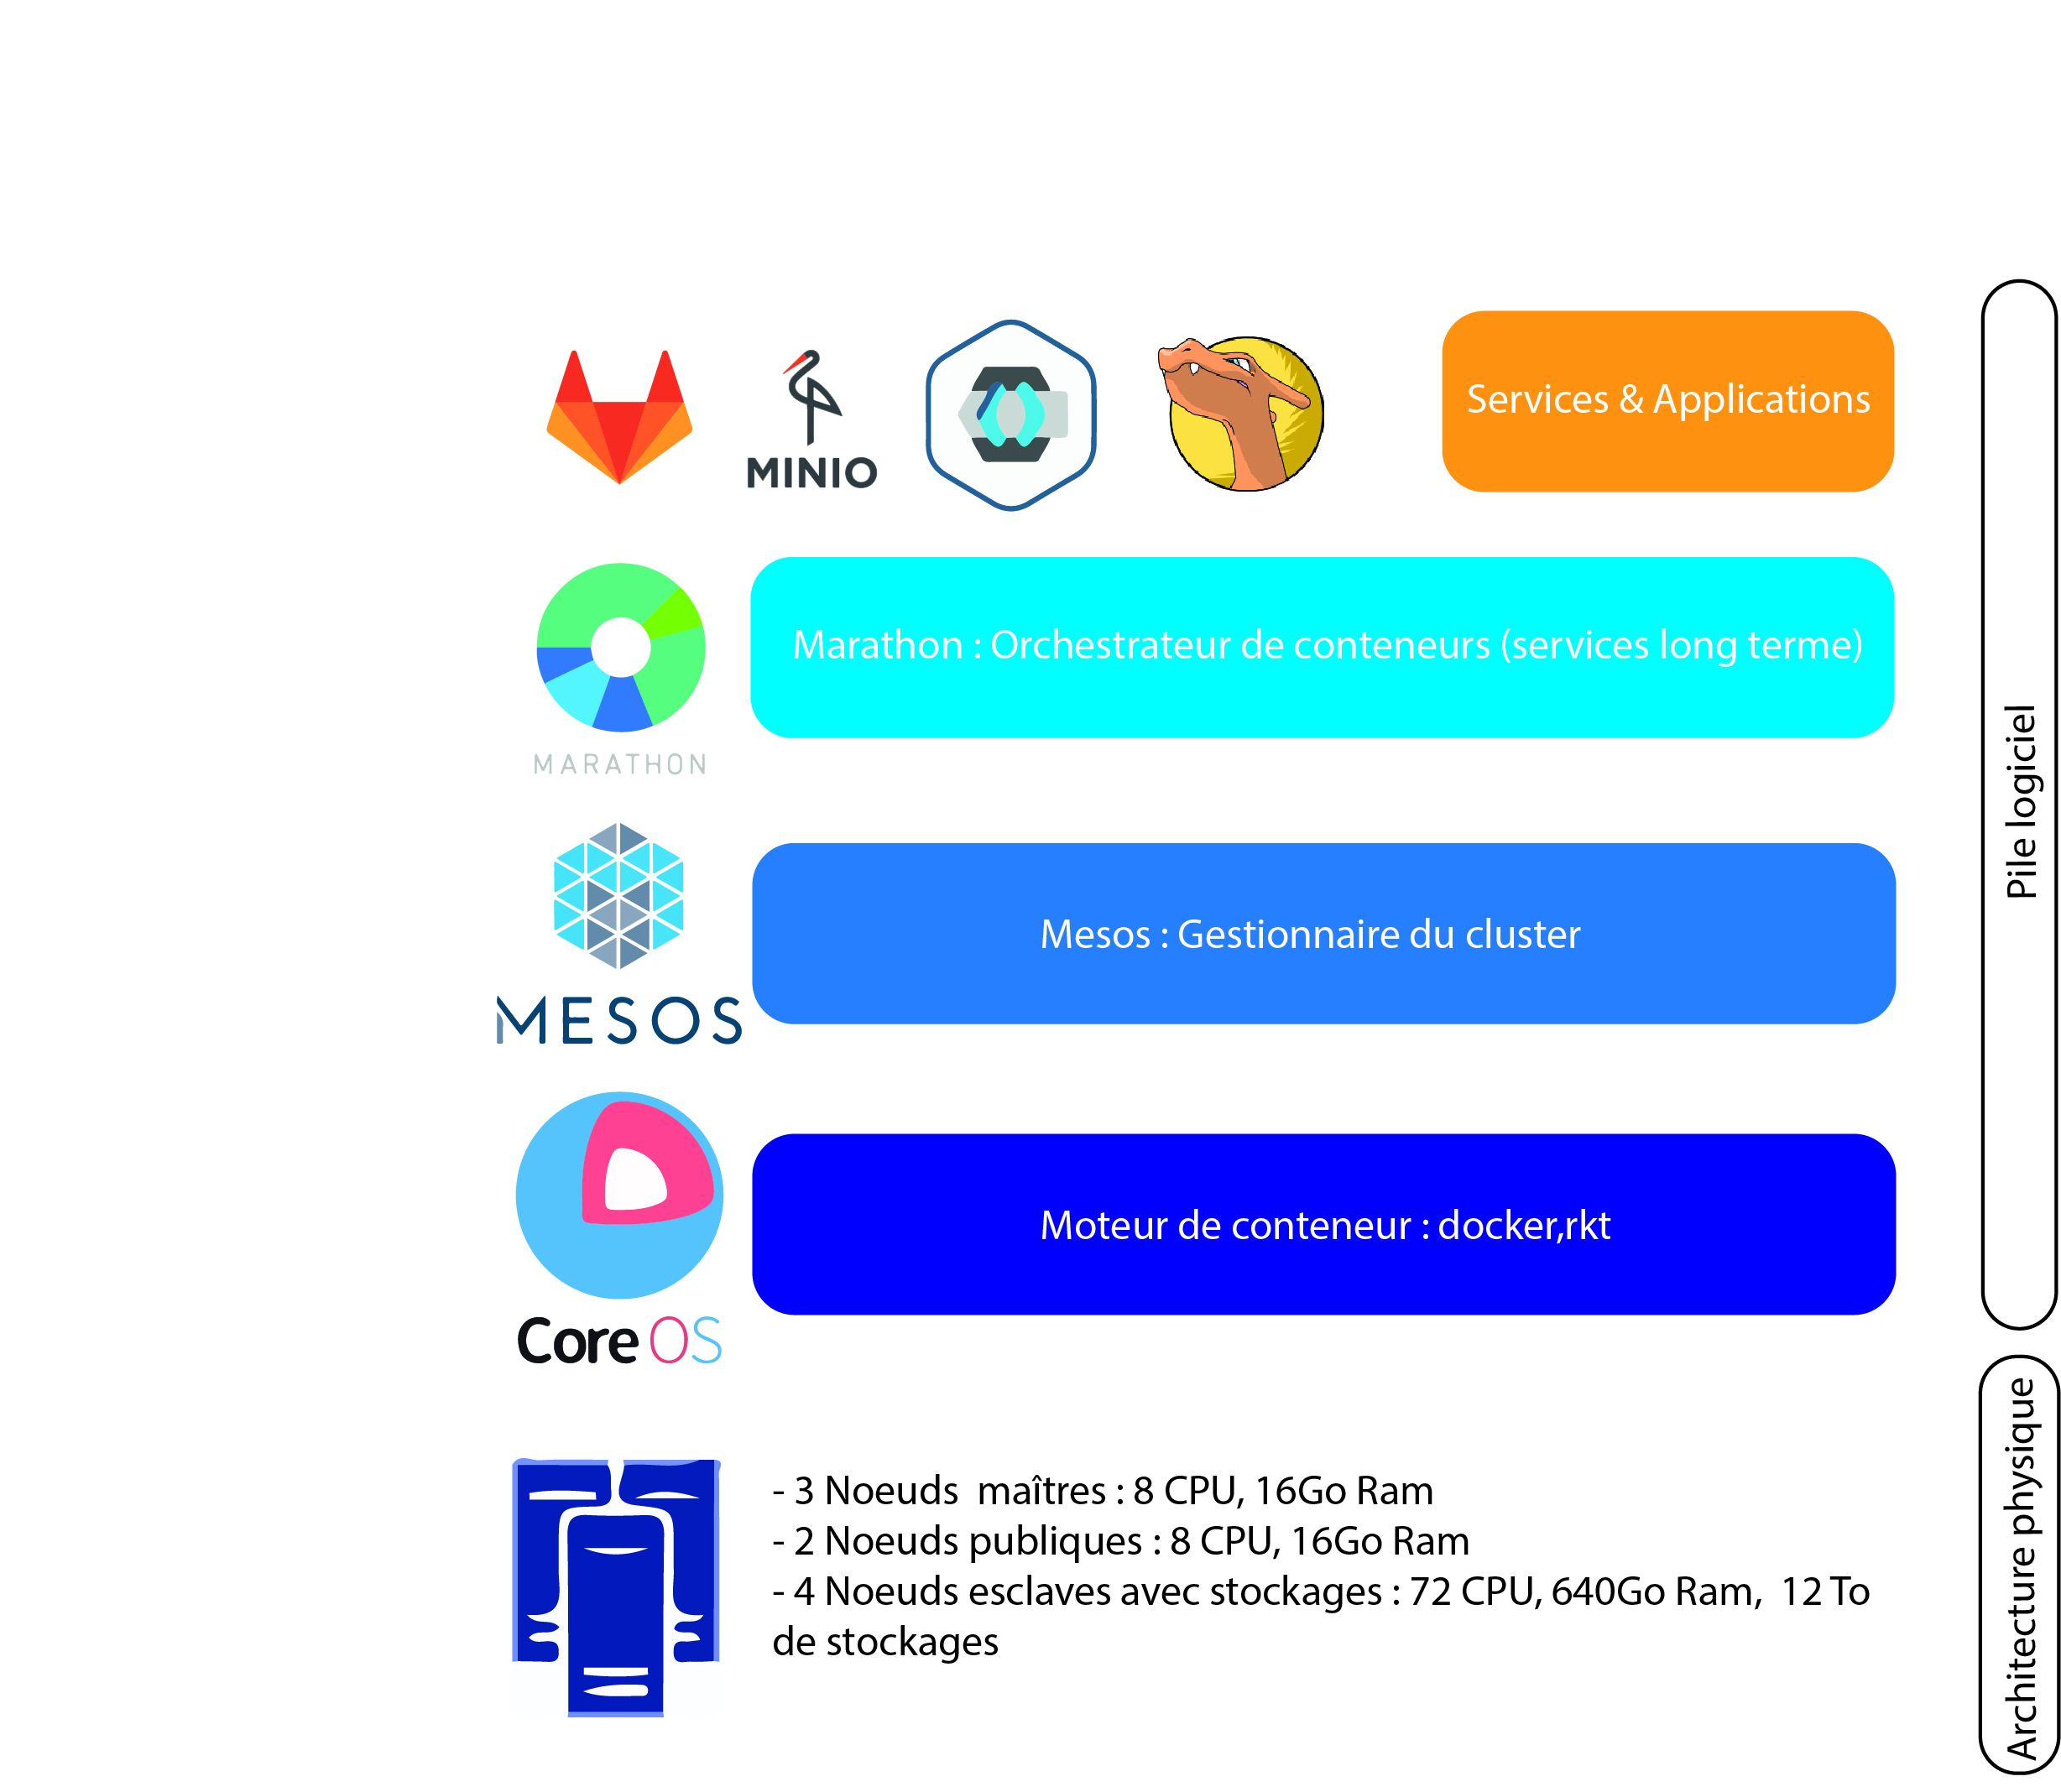
\includegraphics[scale=0.2,clip,trim={18cm, 0cm, 0cm, 11.6cm}]{Pictures/onyxia/Onyxia archi.jpg}
\captionsetup{margin=1.5cm,format=hang,justification=justified}
\caption[]{Schéma simplifié de la plateforme Onyxia \newline}
\end{figure}

Une architecture de type conteneur n'est pas un standard à l'Insee, l'infrastructure de production étant uniquement basée sur des VMs (Virtual Machine ou Machine Virtuelle). L'objectif de mon stage sera donc d'étudier les intérêts de la mise en place d'une architecture conteneurisée pour de l'intégration continue ou du service en self-déploiement. Tout d'abord, nous étudierons les différences entre VM et conteneur afin de comprendre en quoi une architecture conteneurisée peut être un atout. Par la suite, nous verrons qu'une telle architecture se doit de reposer sur un orchestrateur de conteneur. Ce qui nous amènera à faire la comparaison des deux orchestrateurs de conteneurs les plus utilisés actuellement : Marathon (solution utilisée par la plateforme de l'innovation) et Kubernetes. Pour cela, nous nous appuierons notamment sur ce que les deux orchestrateurs peuvent proposer dans le cadre de l'intégration-continue, de services en self-déploiement, ainsi qu'en terme d'aide au développement et de sécurité.


\chapterimage{chapter-image/orchestrateur-01.jpg} % Chapter heading image
\chapter{Orchestrateurs et conteneurs}
\vspace{-2cm}

Afin de comprendre l'intêret des conteneurs, repartons dans le passé et étudions comment une application était initialement déployée.

\section{Du serveur physique au conteneur, évolution}
\subsection{Serveur physique}
Initialement (avant les années 1970 et jusqu'au début des années 2000 à l'Insee), une application était installée sur un un serveur physique. On créait alors les environnements avec des batchs\footnote{Un batch désigne l'automatisation d'une suite de commandes exécutées en série sur un ordinateur sans qu'il soit nécessaire qu'un opérateur intervienne pour réaliser cette opération.}, que l'on lançait manuellement. Les applications était déployées sur le même OS (Operating System ou système d'exploitation) sur un seul Hardware\footnote{Machine physique}. On n'avait donc aucun moyen de limiter les ressources utilisées par une application. Par exemple, si sur une machine nous avions deux applications A et B, si A utilisait trop de ressources alors B avait des performances médiocres. La solution aurait été de n'installer qu'une application par serveur, mais cela aurait conduit à des ressources non utilisées et un coût élevé pour les entreprises. \newline
\begin{wrapfigure}[15]{r}{0.3\textwidth}
    \renewcommand{\figurename}{Diagramme}
    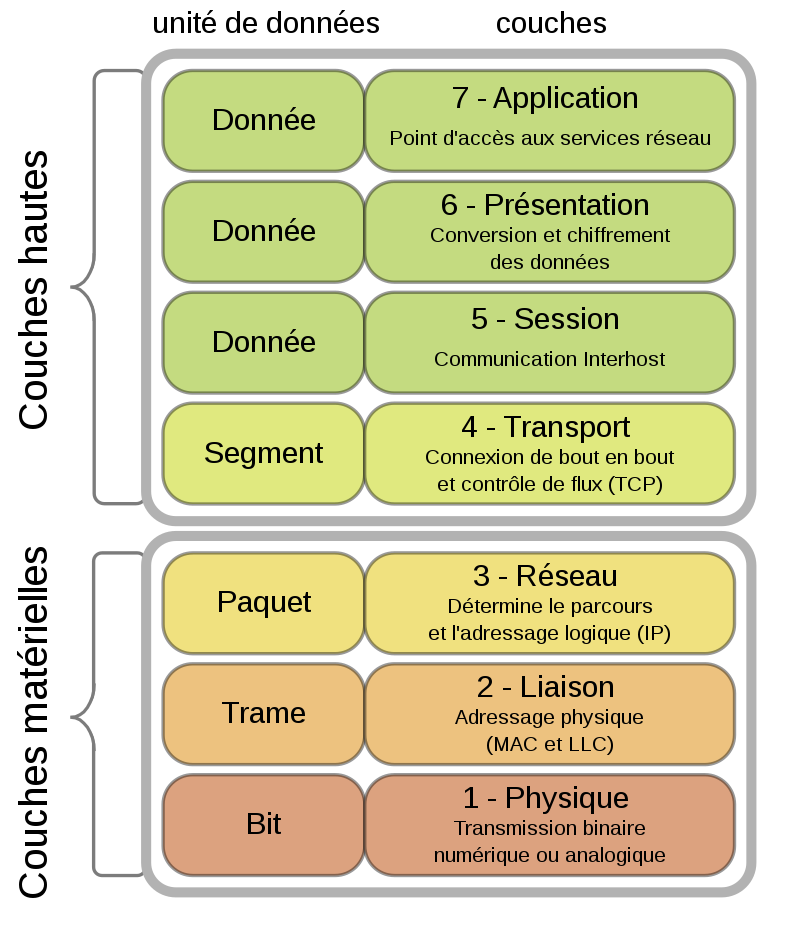
\includegraphics[scale=0.2]{Pictures/OSI.png}
\end{wrapfigure}
\subsection{Virtualisation}
Dans un système d'information, plusieurs applications cohabitent et il est nécessaire que les applications soient indépendantes les unes des autres. Les solutions dites de virtualisation permettent de transformer une ressource physique en un ensemble de ressources logiques isolées. Il est ainsi possible de virtualiser entre autres un réseau ou une machine physique. On fait ainsi fonctionner plusieurs “machines” logiques sur une même machine physique appelée hôte. La virtualisation permet de rendre indépendantes les couches basses (ou matérielles) d’une ressource de ses couches hautes (voir modèle OSI si contre) : les couches hautes peuvent ainsi être aisément déplacées sur une autre infrastructure (en cas de panne ou si les ressources deviennent insuffisantes par exemple).
\paragraph{Les Machines virtuelles}
A partir de 1970 (et au début des années 2000 à l'Insee), apparaît  la notion de machine virtuelle (VM). Les VMs sont des serveurs logiques entiers qui embarquent leur propre système d’exploitation. L’hyperviseur est un applicatif tournant sur l’hôte qui va émuler (ou simuler) le matériel pour la machine virtuelle : le noyau du système d’exploitation de la machine virtuelle croit communiquer avec le matériel de la machine alors qu’il communique avec l’hyperviseur.

Avec le développement des machines virtuelles, de nouveaux outils sont apparus au cours des années 2000/2010 (tel que Puppet\footnote{Puppet est un logiciel libre permettant la gestion de la configuration de serveurs : \url{https://puppet.com/}} ou rundeck \footnote{Rundeck est un logiciel libre permettant l'automatisation d'administration de serveurs via la création de jobs ou tâches. \url{https://www.rundeck.com/open-source}}), qui permettent notamment de configurer automatiquement et rapidement les VMs.


\paragraph{Les conteneurs}
Un conteneur est une unité logicielle standardisée qui regroupe le code, les dépendances, les binaires et l'environnement nécessaires au bon fonctionnement de l'application. Par conséquent, un conteneur est un "package" facile à déplacer d'un environnement à l'autre puisque tout l'écosystème et tout le code est présent à l'intérieur de ce conteneur. Un autre avantage est que, peu importe où s'exécute l'application, le fonctionnement sera identique puisque l'écosystème vient avec le conteneur. Cela permet notamment que l'application se comporte de la même façon, à la fois sur le poste du développeur, que sur un cloud privé ou public. \\




\begin{figure}[H]\centering
\renewcommand{\figurename}{Graphique}
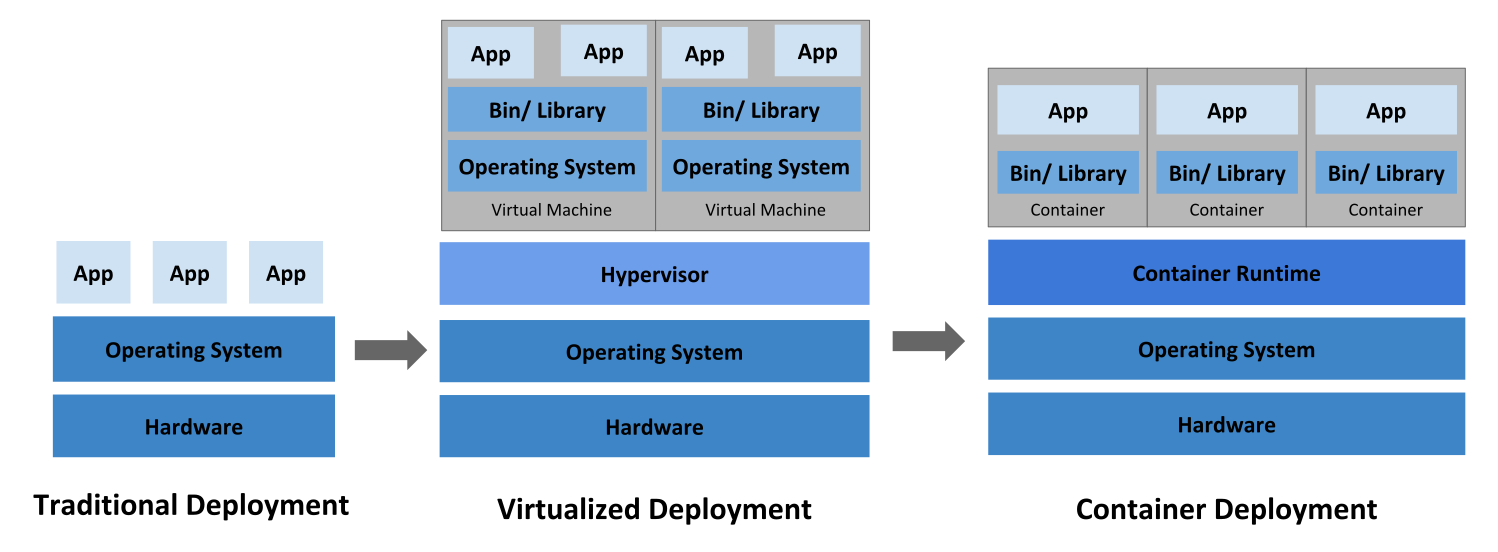
\includegraphics[scale=0.3]{Pictures/container_evolution.png}
\captionsetup{margin=1.5cm,format=hang,justification=justified}
\caption[]{schéma récapitulatif entre VM et conteneur \newline}
\end{figure}


\section{VM ou conteneur: Lequel choisir en 2020 ? }
Les machines virtuelles comme les conteneurs proposent chacun une solution pour virtualiser des ressources et exécuter des applications. Nous allons aborder ici, divers aspects qu'il faut prendre en compte, avant de s'orienter vers l'une des deux solutions.

\paragraph{Choix du système d'exploitation}
Dans le cadre des VMs, l'administrateur a le choix du système d'exploitation utilisé par chacune des VMs. En effet, chaque VM possède son propre système d'exploitation, il est indépendant des autres OS des VMs installées sur la même machine, et il est même indépendant de l'OS du système hôte. De son coté, le conteneur utilise le système d'exploitation du système sur lequel il est déployé et cet OS est partagé avec l'ensemble des conteneurs qui s'exécutent sur la machine. Les machines virtuelles sont donc plus flexibles sur ce point-ci.

\paragraph{Taille d'une application}
Par ailleurs, cette flexibilité des VMs s'accompagne d'une taille bien plus importante. En effet, un iso\footnote{\textcolor{red}{à définir}} a une taille plus importante qu'une image. Pour une VM, il faut packager l'OS, les librairies et l'application ; alors que pour un conteneur, seuls sont nécessaires les librairies et l'application. Ce phénomène s'accentue d'autant plus que l'on veut un nombre de réplicas\footnote{\textcolor{red}{à définir}} élevés.

\paragraph{Rapidité de démarrage}
De même, les conteneurs démarrent bien plus rapidement qu'une machine virtuelle.
Selon l'étude \textit{Comparative Study of Virtual Machines and Containers for DevOps Developers\footnote{\url{https://www.researchgate.net/publication/327237114_Comparative_Study_of_Virtual_Machines_and_Containers_for_DevOps_Developers/citation/download}}}, un Ubuntu met 40 ms pour démarrer et 29 ms pour s'arrêter à partir d'un conteneur, contre près de 59 s pour démarrer et 30 s pour s'éteindre sur une VM.

\paragraph{Rapidité d'écriture des données}
Cette même étude montre également que la vitesse d'écriture et de lecture de données depuis un conteneur est plus rapide que depuis une VM. En effet, un Ubuntu dans un conteneur effectue quasiment autant d'opérations de lecture et d'écriture qu'un Ubuntu installé directement sur une machine.

\paragraph{Sauvegarder, restaurer, migrer}
VirtualBox, Vmware ou encore KVM proposent des solutions afin de réaliser des sauvegardes et/ou de restaurer des machines virtuelles à partir de sauvegardes. Dans le monde du conteneur de telles solutions sont quasi inexistantes \footnote{(CRIU)}, puisque une application s'exécutant dans un conteneur n'a pas vocation à vivre éternellement. (On verra plus loin que les conteneurs peuvent être arrêter et redémarrer plusieurs fois par jour par les orchestrateurs de conteneurs.)

\paragraph{Sécurité}
Cependant, les machines virtuelles offrent une plus grande sécurité. En effet, si un attaquant arrive à sortir de l'application (et à avoir accès à la couche supérieure), dans le cadre d'une VM ce dernier aura accès au BIOS, au réseau de la VM, mais il ne pourra pas accèder aux autres VMs (même celles de la même machine). Les conteneurs n'offrent pas cette isolation, un attaquant qui sortirait de l'application s'exécutant dans le conteneur pourrait alors accéder aux librairies partagées et donc accéder aux autres conteneurs. Cette faille pouvant être causée aussi bien par le développeur que par les dépendances qui auront servis à construire l'image.\footnote{\url{https://www.lemondeinformatique.fr/actualites/lire-une-faille-dans-runc-rend-vulnerable-docker-et-kubernetes-74312.html}} 

\begin{interrupt}
\paragraph{Comment choisir ?}
Dans le cadre de la plateforme innovation et la mise en place de processus de type devOps ou de self-service, on recherche une solution de virtualisation qui soit rapide à  déployer, légère, facilement jetable et facile à reproduire. Les conteneurs semblent donc être la solution idéale, malgré les problèmes de sécurité, puisqu'ils peuvent être facilement réduits \footnote{La sécurité avec Kubernetes et les conteneurs Docker : une histoire sans fin (A. Roman \& C. Dubois) : \url{https://www.youtube.com/watch?v=EEuV_mgRNsY&t=2196s}}. 
\end{interrupt}

\section{Qu'est-ce qu'un orchestrateur ? }
Les architectures applicatives modernes prônent le découpage des applications en modules de petite taille, répondant à un besoin fonctionnel ou technique bien identifié. Ces modules doivent être, dans la mesure du possible, indépendants du système qui les exécute, pour ne conserver que des dépendances logiques entre eux. La notion à la mode est celle d’architecture microservices. Cette notion d'architecture microservice a entrainé une augmentation du nombre de conteneurs déployés afin de faire fonctionner un seul service. Il a donc fallu créer un outil capable de gérer un ensemble de conteneurs : l'orchestrateur de conteneurs.\\ 

La mission d'un orchestrateur de conteneurs est de répartir les conteneurs sur un ensemble de machines. Un orchestrateur de conteneurs est composé de 3 ensembles de machines :
\begin{itemize}
    \item Les workers nodes: ce sont les machines sur lesquels s'exécuteront les conteneurs, ce sont généralement les machines les plus puissantes du cluster. Chacune de ces machines héberge le moteur d'exécution \footnote{Un environnement d'exécution ou runtime est un logiciel responsable de l'exécution des programmes informatiques écrits dans un langage de programmation donné} ainsi qu'un agent qui communique avec les masters nodes.
    \item Les masters nodes : ce sont les machines qui vont gouverner le cluster, qui vont gérer l'ensemble des ressources disponibles (RAM, CPU, GPU, espace disque) sur chaque worker. C'est également le master node qui a les responsabilités de relancer les conteneurs défaillants. C'est généralement le point d'entrée du cluster pour les développeurs.
    \item Les publics nodes :  ce sont les machines exposées sur internet. Elles vont servir de relais entre internet et l'intérieur de notre plateforme. Ces dernières jouent le rôle de reverse proxy.\\
\end{itemize}
 
L'orchestrateur permet donc d'assurer un rôle de surveillant de l'état des conteneurs. En effet, à partir d'un fichier descriptif qui contient le nombre de conteneurs souhaités, l'état désiré, etc... et à l'aide de healtcheck\footnote{\textcolor{red}{à définir}} régulier, il est capable de détecter les conteneurs en mauvaise santé afin d'en démarrer de nouveaux et de toujours maintenir le système dans un état de fonctionnement optimal.\\
Il est aussi capable de tenir compte des contraintes dynamiques : en effet, les contraintes évoluent dans le temps. Par exemple, on peut vouloir que deux conteneurs ne soient jamais sur le même serveur pour garantir une haute disponibilité de services, ou encore, on peut vouloir que les conteneurs soient déployés sur des serveurs éloignés afin de limiter la latence pour l'utilisateur. L'orchestrateur sait également réagir en cas de perte d'une des machines. Il permet donc de mettre en place des mécanismes de haut niveau : haute disponibilité, monitoring, le Service Discovery \footnote{Service Discovery est un protocole réseau qui permet la découverte de service.} et la gestion du trafic réseau,  scalabilité horizontale et verticale, le provisionning et le placement des conteneurs.\\



\section{Les différents orchestrateurs}
Aujourd'hui, plusieurs solutions d'orchestration existent, mais trois se démarquent : Kubernetes, DC/OS avec Mesos/Marathon et  Docker Swarm.

\subsection{Mesos/Marathon}
Mesos est la solution la plus ancienne parmi les trois citées. Développée initialement par Mesosphère (qui est devenu DC/OS puis récemment D2IQ), sa genèse remonte à une époque où la popularité des conteneurs était nettement moindre. Le concept de Mesos est de regrouper un ensemble de ressources (RAM, CPU) pour proposer une vue agrégée, permettant d’exécuter des programmes (conteneurisés ou pas). Mesos n’a pas vocation à être utilisé seul. Il délègue l’exécution des programmes à ses frameworks\footnote{Voir plus loin}. Parmi eux, les plus utilisés sont certainement Marathon et Aurora. Ce sont eux qui, sur la base d’un fichier JSON, sont responsables de placer les conteneurs et de garantir leur exécution dans les conditions souhaitées.\\
C'est la solution actuellement utilisé sur la plateforme de l'innovation pour manager les différentes ressources : service à la demande, gitlab, job gitlab\footnote{\textcolor{red}{à définir}}, etc... \\ 

\subsection{Kubernetes}
Kubernetes (souvent abrégé k8s) est un produit open source développé initialement par Google, et reversé à la communauté. Le géant de l’Internet, à l’origine du développement des cgroups\footnote{cgroups (control groups) est une fonctionnalité du noyau Linux pour limiter, compter et isoler l'utilisation des ressources (processeur, mémoire, utilisation disque, etc.).}, utilise les conteneurs depuis près de 15 ans. Le partage de son orchestrateur avec la communauté constitue donc un gage de qualité. 

\subsection{Swarn Docker}
Swarm est la solution d’orchestration fournie par Docker. Il est difficile de prédire ce que sera Swarm dans un an tant son évolution a été rapide dernièrement. Au départ un composant à part, Swarm est désormais complètement intégré au service Docker. On ne parle plus de Swarm en tant que tel mais du Docker “swarm mode”.\\


Pour cette étude, nous nous intéresserons plus particulièrement à Mesos/Marathon (solution actuellement en place à l'Insee sur la plateforme innovation) et Kubernetes, le nouveau leader mondial dans l'orchestration de conteneur. Selon Sysdig \footnote{\url{https://sysdig.com/blog/sysdig-2019-container-usage-report/}} plus de 77\% des personnes qui utilisent un orchestrateur de conteneur utilisent Kubernetes, et ce taux monte à plus de 85\% si l'on ajoute les solutions openshift et rancher (basées sur Kubernetes). Par ailleurs, Kubernetes bien qu'étant l'orchestrateur de conteneur le plus récent, possède déjà le plus grand nombre de commits et un très bon indice de community performance (nombre de commits par contributeur par an). Nous essayerons de comprendre pourquoi ce petit nouveau entraîne une telle hype avec lui.
\begin{figure}[H]\centering
\renewcommand{\figurename}{Graphique}
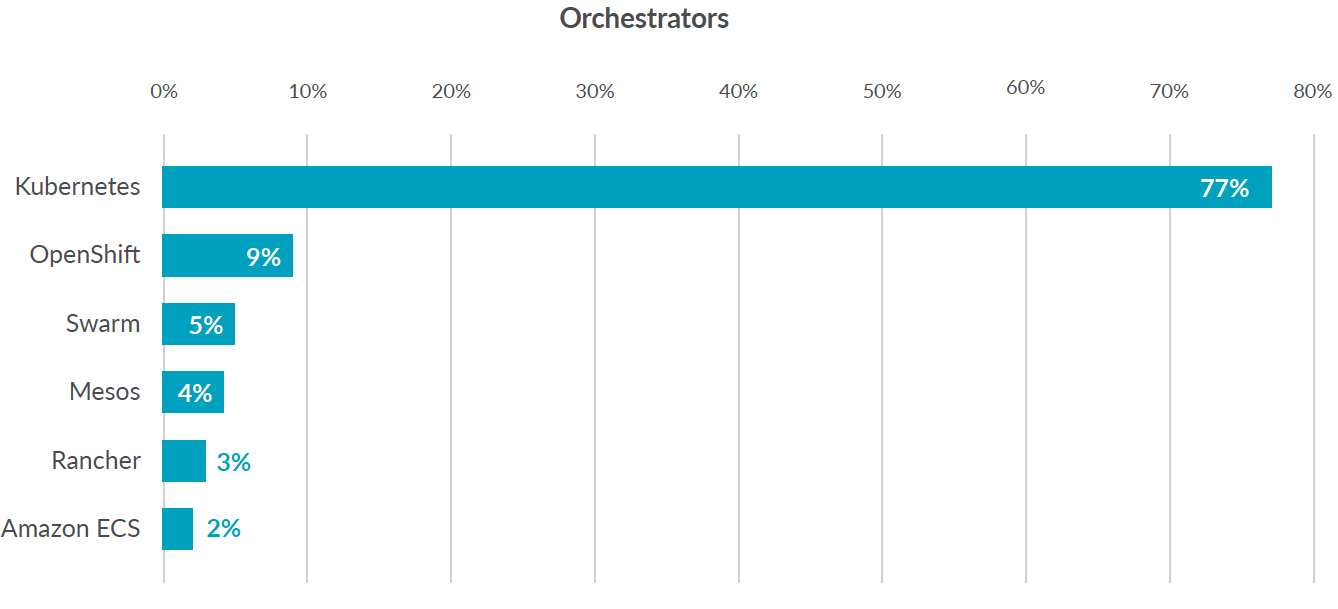
\includegraphics[scale=0.3]{Pictures/orchestrators-2019.png}
\captionsetup{margin=1.5cm,format=hang,justification=justified}
\caption[]{Pourcentage d'utilisation de chaque orchestrateur\newline
Source : Sysdig, \url{https://sysdig.com/blog/sysdig-2019-container-usage-report/}}
\end{figure}


%----------------------------------------------------------------------------------------
%	CHAPTER 2
%----------------------------------------------------------------------------------------
\part{\color{ocre}\textsc{Mesos vs Kubernetes} : Marathon à bout de souffle ?}
\chapterimage{chapter-image/architecture-01.jpg} 
\chapter{Architecture et fonctionnement}
\vspace{-2cm}

Nous allons, dans cette partie, aborder l'architecture d'un cluster Kubernetes et celle d'un cluster Mesos.



\section{Architecture d'un cluster Kubernetes}
Un cluster Kubernetes a obligatoirement au moins un worker node. Le worker node est le serveur qui bénéficie de la plus grosse configuration en termes de CPU, mémoire, RAM puisque c'est lui qui fait tourner les conteneurs (et donc les applications).\newline 

Le control plane gouverne les worker-nodes (et donc les Pods\footnote{Un Pod est un groupe d'un ou plusieurs conteneurs (comme des conteneurs Docker), ayant du stockage/réseau partagé, et une spécification sur la manière d'exécuter ses conteneurs.}) du cluster. Dans les environnements de production, le control plane tourne sur plusieurs machines et le cluster est composé de plusieurs worker nodes, qui sont, dans le cas idéal, répartis géographiquement pour garantir une  meilleure disponibilité de services (et de qualité).\newline

Nous ne parlerons pas ici des public nodes.


\subsection{Les composants du control-plane}
Les composants du control plane (qui correspond au Master-node) sont ceux qui gèrent l'état global du cluster, qui détectent et réagissent en fonction des événements au sein du cluster (déploiement d'une nouvelle application ,load-balancing\footnote{\textcolor{red}{à définir}}, etc...). De manière générale, même si les composants du control plane peuvent être installés sur différentes machines, les scripts classiques déploient l'ensemble des composants du control-plane sur une seule et unique machine, sur laquelle aucun conteneur créé par un utilisateur ne peut être lancé.

\paragraph{Etcd}
Le Master node possède une base de données clés valeurs, où est stocké l'état du cluster Kubernetes. Elle est appelée etcd.

\paragraph{Kube-apiserver}
L'api-server est le composant du Kubernetes control-plane qui expose l'API de Kubernetes. L'api-server est donc le point d'entrée pour l'ensemble des opérations à exécuter sur le cluster, elle fait office de passerelle vers le cluster. Elle reçoit des requêtes REST, elle les valide et met à jour les objets correspondants dans l'etcd. Par définition, l'api-server doit être accessible par des clients extérieurs au cluster. Alors que les nodes, et donc les conteneurs, peuvent ne pas l'être. L'api-server peut aussi être utilisée comme un proxy/tunnel vers les nodes et les Pods.


\paragraph{Kube-controller manager}
Le kube-controler manager est le composant qui contrôle l'état du cluster en continue. Dans le monde de Kubernetes, un contrôleur est un processus qui tourne en boucle : il interroge l'api-server qui lui renvoie l'état du cluster et il effectue les changements (toujours en passant par l'api-server) de manière à ce que le cluster tende toujours vers l'état désiré. Kubernetes possède 4 contrôleurs (initialement, mais on peut en rajouter pour d'autres besoins\footnote{Afin d'exposer nos services, on a besoin d'ingress. L'ingress-controller permet par exemple de scanner l'ensemble des objets ingress et de les ajouter à sa pile.}), regroupés en un seul contrôleur: le controller-manager. Ce dernier regroupe les 4 contrôleurs suivants: 
\begin{itemize}
    \item Node Controller : c'est le contrôleur qui détecte les nodes en pannes et qui agit en conséquence.
    \item Replication Controller : Il vérifie si le cluster contient bien le bon nombre de Pods pour chaque objet ReplicationController (attention on parle ici de l'objet replicationController\footnote{Un replicationController est un objet qui décrit, pour un déploiement donné, combien de réplicas d'une application sont nécessaires} et non du contrôleur en lui même).
    \item Endpoints Controller: Il définit les objets Endpoints (c’est-à-dire les Services qui sont reliés aux Pods).
    \item Service Account et Token Controllers : C'est la partie responsable de la création des comptes par défaut et des jetons d'accès à l'API pour les nouveaux namespaces\footnote{\textcolor{red}{à définir}}.
\end{itemize}

\paragraph{Le cloud-controller manager\footnote{Plus d'informations ici : \url{https://kubernetes.io/fr/docs/concepts/overview/components/\#cloud-controller-manager}}}
Ce composant permet de lier le cluster Kubernetes à la logique du provider cloud. C'est une surcouche qui n'est pas toujours présente (notamment dans le cas d'une installation dite on-premise). Il permet notamment au provider cloud d'ajouter des routes dans le cluster (à la manière d'un reverse proxy). Il ajoute également un volume-controller afin de pouvoir créer des Volumes et interagir avec le fournisseur cloud pour les orchestrer.

\paragraph{Le kube-scheduler}
Le kube-scheduler est le composant du master node qui est responsable de la surveillance des Pods qui viennent d'être créés. En effet, Kubernetes autorise les utilisateurs à lancer sur le cluster des conteneurs. Le kube-scheduler choisi automatiquement quel(s) node(s) va accueillir le ou les conteneurs nouvellement créé(s). Le scheduler détecte les Pods qui ne sont pas affectés, et il les associe à des nodes par le biais de l'api-server, en fonction des besoins et des ressources disponibles.

\subsection{Les composants du Node}
Chaque composant que nous allons voir ici, est exécuté sur chaque node. Ils maintiennent les Pods en vie et fournissent l'environnement d'exécution Kubernetes. Les nodes sont parfois aussi appelés worker-nodes.

\paragraph{Le Kubelet}
Le kubelet est le principal composant qui s'exécute sur chaque node. Il peut enregistrer le node auprès de l'api-server en utilisant l'un des éléments suivants : le nom d'hôte, un flag\footnote{\textcolor{red}{à définir}} pour remplacer le nom d'hôte ou une logique spécifique pour un fournisseur de services cloud.

Le kubelet fonctionne en termes de PodSpec. Un PodSpec est un objet YAML ou JSON qui décrit un Pod. Le kubelet prend un ensemble de PodSpecs qui sont fournis par divers mécanismes (principalement par l'api-server) et s'assure que les conteneurs décrits dans ces PodSpecs fonctionnent et sont en bonne santé.

\paragraph{Le Kube-Proxy}
Kube-proxy est un proxy réseau qui s’exécute sur chaque node du cluster et implémente une partie du mécanisme de Service Discovery.

\paragraph{Le Container-Runtime}
Le Container-Runtime est le logiciel responsable de l’exécution des conteneurs.\\


En résumé, on peut schématiser un cluster Kubernetes de la manière suivante :

\begin{figure}[H]\centering
\renewcommand{\figurename}{Graphique}
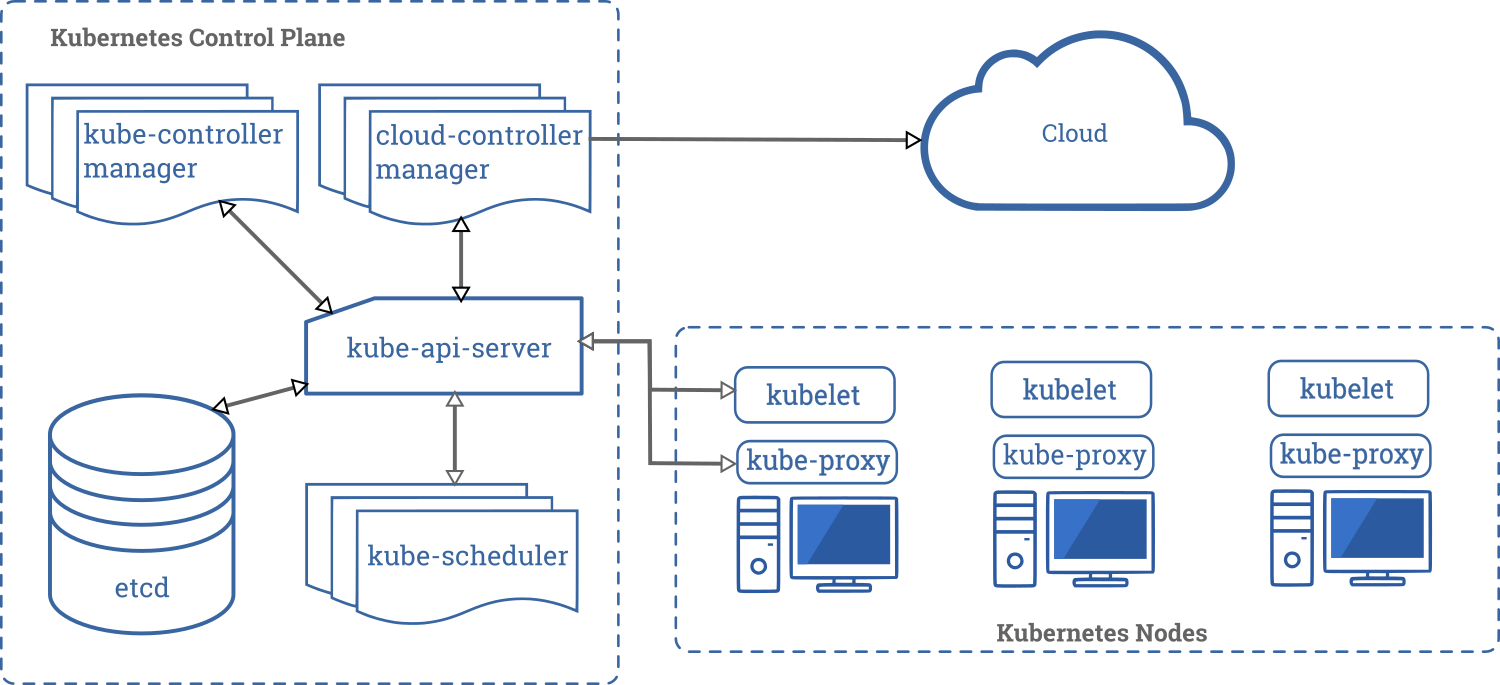
\includegraphics[scale=0.1]{Pictures/Comparaison/Kubernetes-cluster-archi.png}
\captionsetup{margin=1.5cm,format=hang,justification=justified}
\caption[]{Schéma récapitulatif des entitées présentes dans un cluster Kubernetes \newline}
\end{figure}



\begin{interrupt}
\paragraph{Conclusion:}
Un cluster Kubernetes fonctionne de la manière suivante :
sur chaque noeud, on retrouve le kubelet et le kub proxy qui font l'instanciation entre notre image local et l'abstraction du serveur local. Le kubelet communique avec l'api-server afin de communiquer son état que l'API va stocker dans l'etcd.
L'api Server recoit les requêtes, elle vérifie les commandes envoyées à l'aide du controller manager, elle enregistre l'action dans le scheduler qui lui va définir les enfants\footnote{\textcolor{red}{à définir}} et les déploiements.
\end{interrupt}

\section{Architecture d'un cluster Mesos/Marathon}
Tout d'abord, il faut savoir qu'il est impossible d'utiliser l'orchestrateur de conteneur Marathon, sans posséder au préalable un cluster Mesos. Nous allons ici expliquer comment un cluster Mesos fonctionne et comment Marathon s'articule autour de cette architecture.



% control plane c'est du mesos ou kubernetes ??
% - v2 : L'équivalent du control plane est le master node pour un cluster Mesos.
\subsection{Les composants du control plane}
Le control plane est le master node du cluster Mesos. Il abrite deux entitées, le mesos master et les mesos frameworks.
\paragraph{Le mesos master}
Le mesos master est le cœur du cluster. Il garantit la haute disponibilité du cluster. Il héberge l'interface utilisateur qui fournit des informations sur les ressources disponibles dans le cluster. L'API Mesos est accessible par ligne de commande ou directement par requête HTTP. Le master est la source centrale de toutes les tâches en cours, il est la source de vérité dans le cluster. Il stocke en mémoire toutes les données relatives aux tâches, à l'état du cluster. Pour une tâche, il ne stocke que les informations nécessaires, ce qui permet au master de fournir à l'interface utilisateur les données relatives aux tâches avec une latence minimale. C'est le master qui alloue les ressources aux différents frameworks Mesos.

\paragraph{Les schedulers}
Le scheduler est en fait un des deux composants du Framework mesos. Le framework mesos est composé de deux éléments : le scheduler et l'executor. Le premier étant situé dans le control plane et le deuxième dans les mesos slaves rattachés à ce framework. On s'intéresse ici uniquement au scheduler. \\

Lorsqu'il est déployé, le scheduler s'enregistre auprès du master Mesos et obtient un identifiant. A chaque requête reçue par le Mesos master, ce dernier délègue la requête au bon scheduler. Lorsque le scheduleur reçoit la requête, il évalue si il peut satisfaire la demande (par exemple déployer une application) en fonction des ressources que le mesos master met à sa disposition. Il est également responsable de la gestion des échecs et des erreurs des tâches qu'il doit gérer. \\
\paragraph{Marathon}
Marathon est un des scheduler qui peut être déployé dans Mesos. Marathon est même un des piliers de l'architecture des clusters Apache Mesos. Utilisé en production pour l'orchestration de conteneurs, Marathon fournit une API REST pour le démarrage, l'arrêt et la mise à l'échelle des applications. Écrit en Scala, Marathon peut fonctionner en mode haute disponibilité en exécutant plusieurs copies de lui même. L'état des tâches en cours d'exécution est stocké dans la base de données du Mesos master.\\

Marathon est en fait un méta-scheduler, ce qui signifie qu'il peut démarrer d'autres schedulers Mesos tels que Chronos ou Storm. Marathon en tant qu'orchestrateur de conteneur va s'assurer qu'ils survivent aux pannes de machine. Il peut lancer tout ce qui peut être lancé dans un shell standard. (On peut même lancer une autre instance de Marathon via Marathon.)

\subsection{Les composants du mesos slave}
Un cluster mesos est composé de plusieurs mesos slave, c'est l'équivalent des workers nodes. L'ensemble des tâches va donc s'éxécuter sur ces machines. Chaque mesos slave héberge, en plus de lui même, deux composants : le ou les schedulers locaux ainsi que leur executor associé. Le Mesos slave fournit au Mesos master les informations relatives à l'hôte dans lequel il s'exécute (y compris les données sur les tâches en cours, les ressources disponibles de l'hôte qui lui sont allouées et d'autres métadonnées).

\paragraph{Le scheduler local}
Le scheduler local communique avec le Mesos slave. Il garantit la livraison des mises à jour de l'état des tâches aux executors.
\paragraph{L'executor}
L'executor exécute la tâche lancée par le scheduleur (relayée par le scheduler local) et notifie en retour le statut de chaque tâche.


\begin{figure}[H]\centering
\renewcommand{\figurename}{Graphique}
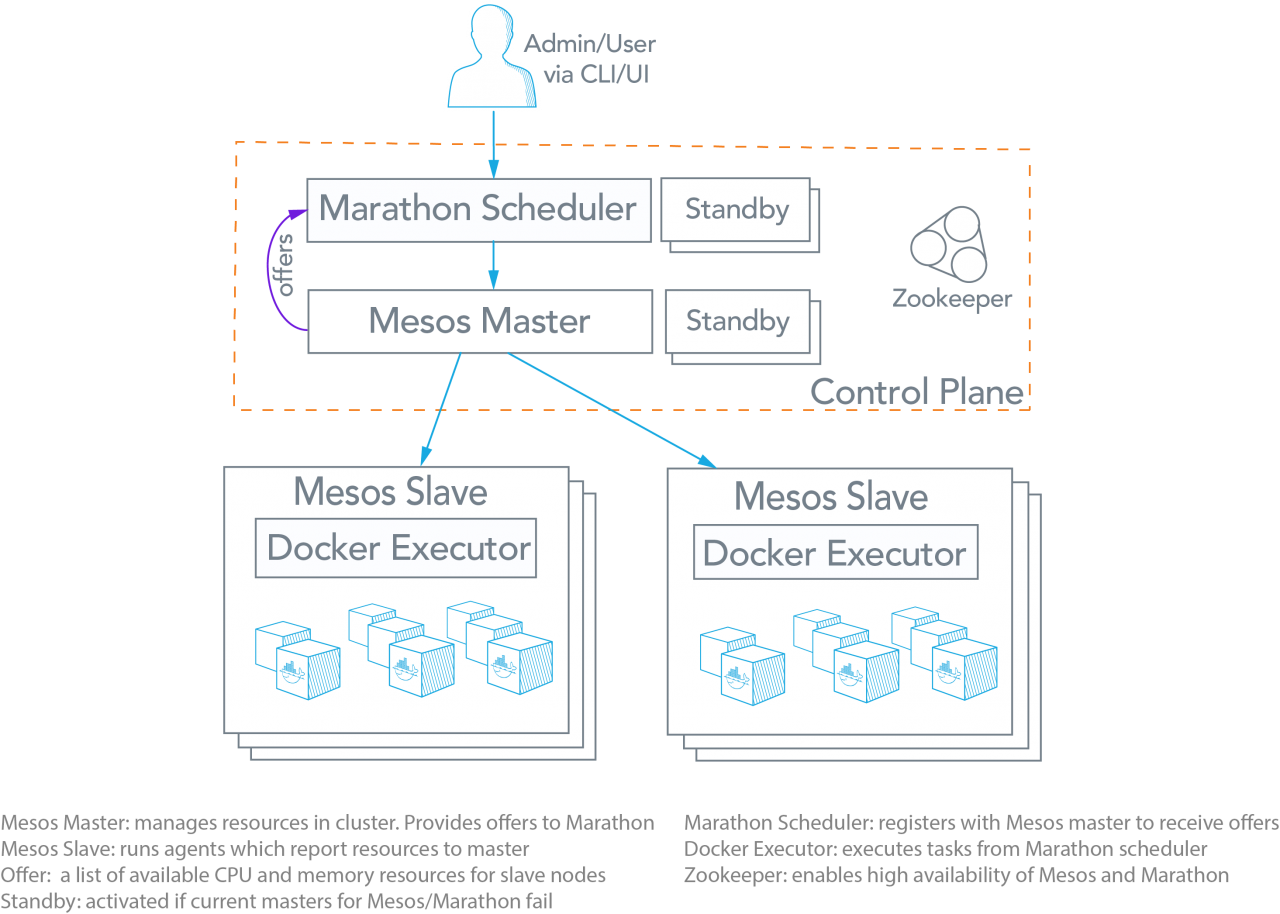
\includegraphics[scale=0.3,trim={0 5cm 0 0},clip]{Pictures/Comparaison/mesos-architecture.png}
\captionsetup{margin=1.5cm,format=hang,justification=justified}
\caption[]{Schéma récapitulatif des entitées présentes dans un cluster Mesos \newline}
\end{figure}

\begin{interrupt}
\paragraph{Conclusion:}
L'architecture de Mesos est donc similaire à celle de Kubernetes. Cependant, Mesos ajoute une couche (les schedulers) qui n'existe pas dans Kubernetes. En effet, un cluster mesos permet de déployer bien plus que uniquement des conteneurs par l'intermédiaire de Marathon. Cependant, cette fonctionnalité complexifie l'architecture du cluster. Par la suite, nous ne tiendront pas compte des autres schedulers que peut fournir Mesos, puisque nous cherchons ici à comparer les orchestrateurs de conteneurs.  
\end{interrupt}
\chapterimage{chapter-image/deployer-01.jpg} 
\chapter{Déployer une application}
\vspace{-2cm}

\section{Déployer une application : 2 approches différentes}
Nous ne présenterons pas ici le code nécéssaire pour le déploiement d'une application (le code de déploiement d'une application dans l'un ou l'autre orchestrateur est présent en annexe), mais les différences entre les deux approches.\\
\paragraph{Marathon}
 Marathon utilise des fichiers JSON pour la configuration des déploiements. La configuration de la tâche s'effectue par l'intermédiaire d'un seul fichier. Dans ce fichier, on retrouve notamment l'image que l'on veut utiliser, l'url sur lequel le service sera rendu accessible, les variables d'environnements qui seront par la suite injectées dans le conteneur, le nombre de réplicas, la limitation de CPU et/ou de mémoire. Il existe également une balise fetch qui permet à Marathon, lors du déploiement du service, d'aller récupérer un ou plusieurs fichiers et les ajouter directement au conteneur. L'envoi de ce fichier à Marathon se fait par l'intermédiaire d'une requête POST sur le endpoint v2/deployments.
\paragraph{Kubernetes}
Kubernetes utilise des fichiers yaml pour la configuration des déploiements. Un déploiement est l'assemblage de plusieurs fichiers (qui sont en fait la description de ressources). Lors d'un déploiement, l'utilisateur doit configurer au moins 3 fichiers : le déploiement, le service, et l'ingress. Le premier sert à créer un Pod \footnote{Un Pod est la plus petite unité logique de k8s, encapsule un ou plusieurs conteneurs (dans ce cas il partage le même contexte) Un Pod est attaché à un node, son existence est temporaire, on peut facilement le répliquer sur un autre node. Chaque Pod a une adresse IP virtuelle unique au sein du cluster ce qui permettra aux autres Pods du cluster de communiquer avec ce dernier.} dans notre cluster, ce Pod est situé sur un des nodes, mais il n'est pas accessible (ni de l'intérieur ni de l'extérieur du cluster). Le service \footnote{Un service peut être défini comme un ensemble logique de Pods exposés en tant que service réseau. C'est un niveau d'abstraction au-dessus du Pod, qui fournit une adresse IP et un nom DNS unique pour un ensemble de Pods.} va permettre d'exposer à l'intérieur du cluster ce Pod. Enfin, l'ingress permettra d'exposer ce service au monde extérieur. Cette séparation des fichiers est à la base de Kubernetes. Par exemple, l'ajout de variables d'environnement passe par l'intermédiaire d'une autre ressource : les configMaps.\\

Kubernetes rajoute la notion d'init-container, c'est un container s'exécutant avant celui que l'on veut déployer et qui va permettre de réaliser des actions : téléchargement de données, tests de connexion à certains outils... 

Enfin, Kubernetes permet l'isolation des ressources entre divers utilisateurs, par l'intermédiaire des namespaces. Un namespace est une partition virtuel du cluster Kubernetes. C’est un moyen de diviser un cluster Kubernetes entre plusieurs utilisateurs. Deux ressources au sein du même namespace ne peuvent pas avoir le même nom, mais entre deux namespaces oui. Sauf mention contraire, une ressource d’un namespace ne peut aller interroger directement une ressource d’un autre namespace, cela permet d’isoler les déploiements d’un groupe d’utilisateurs.

\begin{figure}[H]\centering
\begin{tabular}{@{}lll@{}}
\toprule
                             & Marathon       & Kubernetes      \\ \midrule
Fichiers/déploiement         & 1 seul         & Plusieurs       \\
Language                     & Json           & Yaml            \\
Isolation entre utilisateurs & non            & Oui (namespace) \\
Variable d'environnements    & Balise env     & ConfigMap       \\
Télechargement de ressources & Balise Fetch   & InitContainer   \\
Stockage                     & Balise Stockage & VolumeClaim     \\ \bottomrule
\end{tabular}
\caption{Tableau Récapitulatif des points communs et différences entre déploiement Marathon et Kubernetes}
\label{tab:my-table}
\end{figure}


\begin{interrupt}
\paragraph{Conclusion :}
Le déploiement d'une application est donc bien plus verbeux dans Kubernetes que dans le cadre de Marathon. Mais la contrepartie est que cela permet une plus grande finesse dans la configuration des déploiements. Un exemple complet de code permettant de déployer une application dans le cadre des deux orchestrateurs se trouve en annexe A.
\end{interrupt}

\section{Du format de templating au gestionnaire de paquet}

Le principe d'un gestionnaire de paquet est de pouvoir faciliter le déploiement d'un service au sein d'un environnement. Par exemple sur Linux si je veux installer wget il suffit d'ouvrir un terminal et taper \textit{sudo apt-get install wget}. Il pourrait donc être intéressant de disposer du même type d'outils mais au sein d'un cluster, pour par exemple installer rapidement des applications tel que keycloak (authentification), la sphère prometheus-grafana, ou encore la brique ELK. Marathon comme Kubernetes propose chacun leur gestionnaire de paquet. Helm pour Kubernetes, Universe pour DC/OS. Nous présenterons ici leur format, leur fonctionnement et comment les utiliser.

\subsection{Universe (DC/OS)}
DC/OS a introduit la notion de Universe pour son gestionnaire de paquet. Universe n'est pas directement un gestionnaire de paquet, mais plutôt un format de templating utilisé par DC/OS pour son gestionnaire de paquet. \newline

Un Universe est un ensemble de paquets qui peuvent être installer au sein du cluster Mesos par le biais de l'interface UI (admin) de DC/OS ou bien par la ligne de commande DC/OS.\newline


Un universe est décrit par un fichier json (exposé ici par exemple \url{https://inseefrlab.github.io/Universe-Datascience/universe.json}). Chaque package est décrit par la fusion de 4 principaux fichiers présent dans le dépot de l'universe: config.json, marathon.json.mustache, ressource.json et package.json.

\begin{figure}[H]\centering
\renewcommand{\figurename}{Graphique}
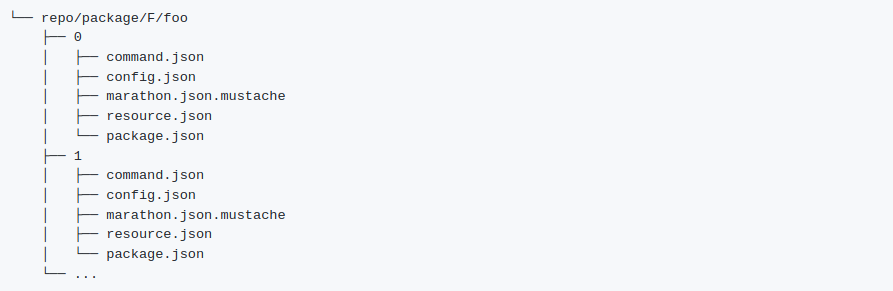
\includegraphics[scale=0.5,trim={0 0 20cm 0},clip ]{Pictures/Comparaison/deployer/universe/universe-repo.png}
\captionsetup{margin=1.5cm,format=hang,justification=justified}
\caption[]{Extrait des fichiers composant un universe \newline}
\end{figure}

\paragraph{marathon.json.mustache:} Ce fichier est le template de l'application, qui une fois complété, créera une définition d'application Marathon capable de faire fonctionner le service. Les variables du marathon.json.mustache seront évaluées à partir d'un objet d'union créé en fusionnant trois objets dans l'ordre suivant :
\begin{itemize}
    \item Valeurs par défaut spécifiées dans le fichier config.json
    \item Les options fournies par l'utilisateur proviennent soit du DC/OS CLI, soit du DC/OS UI
    \item Le contenu de resource.json
\end{itemize}


\paragraph{config.json:} Ce fichier décrit les propriétés de configuration supportées par le package, représenté sous la forme d'un schéma json. Chaque propriété peut spécifier si elle est requise ou non, une valeur par défaut, ainsi qu'une valeur de base.

Les utilisateurs peuvent ensuite remplacer des valeurs spécifiques au moment de l'installation en transmettant un fichier d'options à l'interface utilisateur du DC/OS ou en définissant des valeurs de configuration via l'interface utilisateur du DC/OS.

\paragraph{resource.json:} Ce fichier contient toutes les ressources hébergées en externe (par exemple les images Docker, les images,etc...) nécessaires à l'installation de l'application.

\paragraph{package.json:} Ce fichier contient des informations sur le package en question comme par exemple la version, son nom, etc...\newline 

\subsubsection{Installation}
Le catalogue Universe proposé par DC/OS contient environ 120 paquets que l'on peut exécuter uniquement depuis l'interface admin de DC/OS ou la cli DC/OS.



\subsection{Helm (Kubernetes)}
Helm est un projet opensource créé en 2015. C'est le gestionnaire de paquet recommandé par la CNCF pour l'univers Kubernetes. C'est un projet implémenter en GO (comme de nombreux projet qui gravite autour de Kubernetes).\\

Helm est un SDK (Software Development Kit, un ensemble d’outils d’aide à la programmation) qui se découpe en 2 parties: 
\begin{itemize}
    \item Le client helm qui est une ligne de commande pour l'utilisateur. La ligne de commande permet d'installer ou désinstaller des applications, d'installer automatiquement des dépendances applicatives de mettre à jour des applications, de configurer des déploiements d'application, de récupérer des paquets d'application dans des dépôts, et enfin de communiquer avec la librairie Helm.
    \item La librairie helm fournit la logique pour exécuter les commandes Helm. C'est la partie de Helm qui s'interface avec l'api-server de Kubernetes et qui permet de combiner les templates et la configuration des charts pour créer des releases. C'est également elle qui implémente la logique de montée de version (rolling-update) ou de désinstallation des releases.
\end{itemize}

Helm s'accompagne de 3 concepts : les charts, la config et la release. Nous allons parcourir ces différentes notions.

\subsubsection{Charts}
Les packages Helm sont appelés des charts et sont composés de plusieurs fichiers de configurations yaml (qui sont principalement des templates) et qui seront converti en fichier yaml compréhensible par Kubernetes par la librairie helm. La structure d'un chart est la suivante :

\begin{figure}[H]\centering
\renewcommand{\figurename}{Tableau}
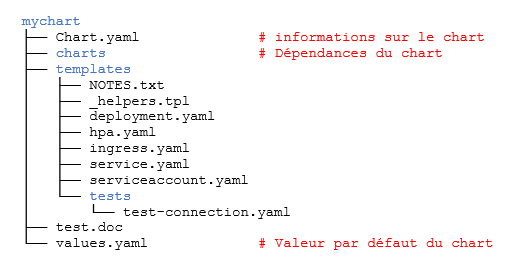
\includegraphics[scale=0.8]{Pictures/Comparaison/deployer/Kubernetes/helmChart.png}
\captionsetup{margin=1.5cm,format=hang,justification=justified}
\caption[]{Aperçus des fichiers composant un chart \newline}
\end{figure}

\begin{itemize}
        \item charts/ : Les dépendances gérées manuellement peuvent être placées dans ce répertoire, bien qu'il soit généralement préférable d'utiliser dependencies dans Chart.yaml pour lier dynamiquement les dépendances.
        \item templates/ : Ce répertoire contient des fichiers templates qui vont être combinés avec des valeurs de configuration (provenant de values.yaml et de la ligne de commande) et rendus dans des manifestes Kubernetes. Ils contiennent en général au moins l'équivalent des trois fichier basique de Kubernetes : ingress service et deployment. Les modèles utilisent le format de template du langage de programmation Go.
        \item Chart.yaml : Un fichier YAML contenant des métadonnées sur le chart, telles que le nom et la version du chart, des informations sur le créateur, un site web pertinent et des mots-clés de recherche, les dépendances du chart.
      \item LICENCE : Une licence en texte clair pour le chart.
     \item README.md : Un fichier readme avec des informations pour les utilisateurs du chart.
      \item values.yaml : Un fichier YAML contenant les valeurs de configuration par défaut du chart.\newline
        \begin{figure}[H]\centering
        \renewcommand{\figurename}{Tableau}
        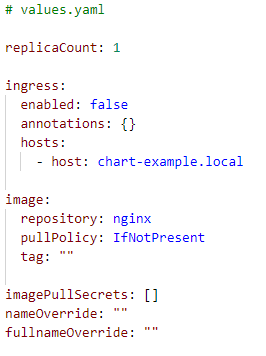
\includegraphics[scale=0.8]{Pictures/Comparaison/deployer/Kubernetes/values.png}
        \captionsetup{margin=1.5cm,format=hang,justification=justified}
        \caption[]{values.yaml \newline}
        \end{figure}
\end{itemize} 
L'ensemble des charts est ensuite placé dans un Helm repository. Un Helm repository est un site HTTP qui sert un fichier index.yaml et des charts packagées. Ces fichiers peuvent être servis par n'importe quel serveur web, service de stockage d'objets ou un hôte de site statique tel que les pages GitHub.

\subsubsection{Config et Release}
Helm permet de surcharger la configuration par défaut fourni avec un chart. Cette surcharge peut s'effectuer de deux manières distincte:
\begin{itemize}
    \item Par le biais d'un fichier values.yaml: l'utilisateur créé un fichier contenant les valeurs qui souhaite surcharger par rapport a la configuration par défaut. Par exemple, si l'on reprends le fichier values.yaml ci-dessus, si l'utilisateur souhaite activer l'ingress, il aura juste à créer un fichier de la forme suivante : 
        \begin{figure}[H]\centering
        \renewcommand{\figurename}{Tableau}
        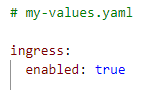
\includegraphics[scale=1]{Pictures/Comparaison/deployer/Kubernetes/my-values.PNG}
        \captionsetup{margin=1.5cm,format=hang,justification=justified}
        \caption[]{my-values.yaml \newline}
        \end{figure}
    Il lui suffit alors de le préciser lors de l'installation du chart \textit{helm install chart mychart -f my-values.yaml}
    \item L'utilisateur peut également surcharger les valeurs de déploiement directement depuis la ligne de commande. On aurait donc (pour le même exemple que ci dessus) \textit{helm install chart mychart --set ingress.enabled=true}.
    \item Enfin on peut également combiner les deux. \textit{helm install chart mychart -f my-values.yaml --set ingress.enabled=true}.
\end{itemize}

Lorsque un chart est installé dans le cluster on parle alors de release. Une release est une instance d'un chart exécuté dans un cluster Kubernetes. Un chart peut souvent être installé plusieurs fois dans le même cluster. Et chaque fois qu'il est installé, une nouvelle release est créée.


\begin{interrupt}
\paragraph{Conclusion:}
La différence avec Universe est frappante. En effet Universe est un format de templating compris et développé par DC/OS pour DC/OS uniquement exécutable depuis l'interface admin de DC/OS (ou depuis la cli mais c'est assez rare) donc assez peu propice a une utilisation massive par plusieurs utilisateurs. Les paquets universes sont en général plutôt utilisé pour déployer des outils d'adminisration du cluster, ou pour déployer des applications en un seul exemplaire. \newline 

Helm quand à lui est une cli qui permet à la fois de déployer des charts dans Kubernetes mais aussi de lister les services déja installés, de faire des upgrades, de créer des charts etc... Et comme universe c'est aussi un outils qui fournit son propre type de templating.\newline

Mais puisque Helm discute avec l'api-server de Kubernetes, il est très facile de faire une politique de gestion de droits, de restreindre un utilisateur a certains workspace, et donc d'avoir plusieurs instance du même chart qui s'éxecute au sein de mon cluster. Par ailleurs Helm est le gestionnaire de packages recommandé par la Cloud Native Computing Foundation, ce qui lui vaut un certains succès. En effet helm propose plus de 1200 charts Helm (bien loin des 120 packages du répertoire DC/OS) qui sont référencé sur \url{https://hub.helm.sh/}. Ce hub contient l'ensemble des charts helm considéré comme stable par Google. Mais il existe aussi de nombreux répertoires Helm alternatif.\newline

Enfin on pourrait reprocher a Helm de ne pas avoir d'interface graphique, mais il existe un chart helm Kubeapps, permettant de donner une UI à Helm pour l'installation de nouveaux charts. 
\end{interrupt}







\chapterimage{chapter-image/git-01.jpg} 
\chapter{CI/CD: Kubernetes un pas vers le GitOps}
\vspace{-2cm}
Actuellement, le cluster Mesos de l'innovation exécuté près de 700 tâches par jour et est utilisé à des fins d'intégration continue et de déploiement d'environnement de tests. Nous allons voir ici ce qu'apporte en plus Kubernetes par rapport à Marathon.

\section{Les prérequis et risques d'une infrastructure conteneurisée}
Avant de se lancer dans le GitOps, il faut d'abord que notre projet réponde à certains critères. On parle alors d'application cloud-Native. La CNCF\footnote{Cloud Native Computing Foundation} donne la définition suivante du cloud-native: \\

\textit{"Les technologies cloud-native permettent aux entreprises de construire et d'exploiter des applications élastiques dans des environnements modernes et dynamiques comme des clouds publics, privés ou bien hybrides. Les conteneurs, les services maillés, les micro services, les infrastructures immuables et les API REST illustrent cette approche. Ces techniques permettent la mise en œuvre de systèmes faiblement couplés, à la fois résistants, pilotables et observables. Combinés à un robuste système d'automatisation, ils permettent aux ingénieurs de procéder à des modifications impactantes, fréquemment et de façon prévisible avec un minimum de travail."} \\

Il faut donc avoir des applications scalables et stateless. Selon une étude réalisée par Sysdig \footnote{\url{https://sysdig.com/blog/sysdig-2019-container-usage-report/}} 25\% des conteneurs s'executant dans un cluster ont une durée de vie inférieure a 10 secondes. Une application monolithique qui stocke ses données en session n'est donc pas adaptée à un déploiement dans le cloud.  \\

Par ailleurs un cluster s'expose au risques suivants: 
\begin{itemize}
    \item Le downtime : Si un conteneur (ou pire un worker-node) contenant une application dysfonctionne pour une raison quelconque, il faut que l'orchestrateur relance cette application. Durant ce laps de temps l'application peut-etre indisponible. Un moyen de palier à ce problème est d'avoir plusieurs répliques de notre application répartis sur plusieurs nodes, pour qu'en cas de bug d'une des répliques, les autres prennent le relais. Il est donc interdit a l'application de posséder des données en local. 
    \item La surcharge : Il peut arriver que le cluster soit en surcharge : suite à la perte d'un node obligeant le déplacement des apps sur un autre node (pertes de ressources entraînant une surcharge), ou encore que l'ensemble des  applications consomme toutes les ressources disponibles. Pour cela on a deux solutions : prévoir large (c'est-à-dire surdimensionner le cluster mais cela entraine une non utilisation des ressources) ou bien faire de l'autoscaling (c'est-à-dire laisser automatiquement le cluster démarrer des worker-nodes ou des conteneurs afin de répondre à la charge, le problème est que cela peut coûter cher). \footnote{C'est d'ailleurs à cause de cette raison que Amazon s'est initialement converti en fournisseur cloud : leur serveur était surchargé pendant certaines périodes de l'année (fêtes de fin d'année). Ils ont donc décidé de louer les ressources qu'ils n'utilisaient pas le reste de l'année, afin de rentabiliser leur infrastructure.}
    \item La perte de donnée : de la même façon que précédemment, aucune donnée ne doit être attachée a un conteneur, il faut donc dans le cas du stockage de données (comme par exemple pour une base de données) avoir une certaine redondance des données et/ou pouvoir les externaliser. Les applications stateless ne possèdent aucune donnée en local, tout leur état étant déporté sur une autre application.
\end{itemize}

Le cloud impose donc de nouvelles manières de développer tel que les microservices, l'event sourcing, le nosql, le stateless, le rest etc...

\section{GitOps: déploiement as code}
Le GitOps est une approche où on décrit l’état de notre infrastructure dans Git. Le répertoire Git contenant la configuration doit contenir l’état souhaité de l’infrastructure. Un opérateur (une application intermédiaire) surveille les modifications dans le répertoire et applique ces modifications pour s’assurer qu’il n’y ait pas d’écart entre l’état souhaité (le contenu du répertoire) et l’état actuel (l’état de l’environnement). 

\begin{figure}[H]\centering
\renewcommand{\figurename}{Graphique}

\includegraphics[scale=0.8]{Pictures/CI-CD/gitops-Intro.png}
\captionsetup{margin=1.5cm,format=hang,justification=justified}
\caption[]{Schéma simplifier du fonctionnement de GitOps \newline}
\end{figure}

Les changements via l’interface utilisateur ou la ligne de commande sont en général interdits. Tout changement doit être approuvé à travers des pull request (ou merge request). Suite à cette approbation, la modification sera appliquée automatiquement par l’opérateur.\\

On retrouve deux modèles pour implémenter le GitOps: le modèle en push et le modèle en pull. Les deux modèles reposent sur la présence de 2 répertoires git : le premier contenant le code, le second contenant les fichiers pour le déploiement. De même les étapes suivantes ont lieu dans les 2 cas: 
\begin{itemize}
     \item Un nouveau commit déclenche le pipeline de build (la partie CI).
    \item Ce pipeline de build package l'application puis lance les tests.
    \item Si les tests passent, alors on construit l'image docker associé à l'application et la push sur le répertoire d'image.
    \item Enfin, le pipeline de CI se termine en pushant sur le repo contenant la configuration, la nouvelle version de l'image à utiliser.
\end{itemize}
C'est par la suite que l'on distingue le modèle en push du modèle en pull
\subsection{Le modèle en push}
\begin{figure}[H]
\renewcommand{\figurename}{Graphique}
\hspace{-2cm}
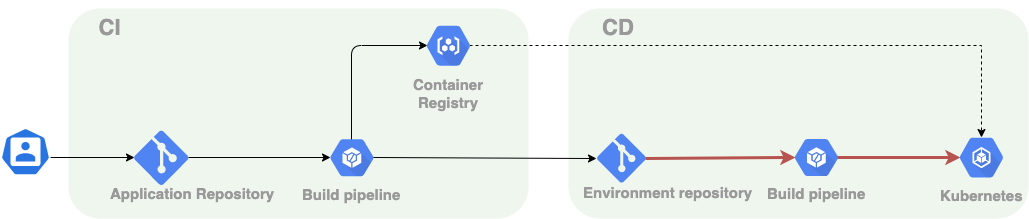
\includegraphics[scale=0.5]{Pictures/CI-CD/push.png}
\captionsetup{margin=1.5cm,format=hang,justification=justified}
\caption[]{Schéma simplifier du modèle push de GitOps \newline}
\end{figure}

Dans le modèle en push, lorsque le répertoire contenant la configuration est mis à jour, un nouveau pipeline se lance afin de pusher la nouvelle configuration vers l'orchestrateur.\\
L'application qui push les changements vers l'orchestrateur joue alors le rôle de l'opérator. Avec ce modèle, on ne peut cependant pas distinguer (sans monitoring ou investigation manuelle) une divergence entre la version s'exécutant dans le cluster et la version du répértoire git. 

\subsection{Le modèle en pull}
\begin{figure}[H]
\renewcommand{\figurename}{Graphique}
\hspace{-2cm}
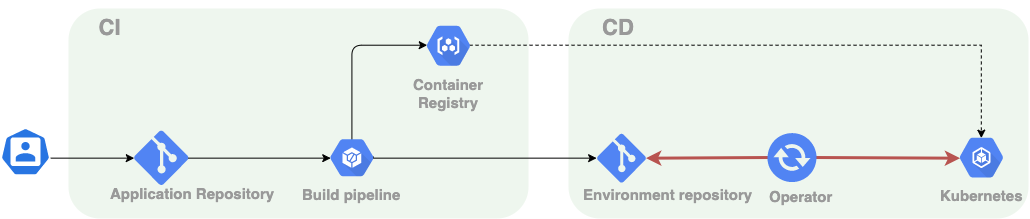
\includegraphics[scale=0.5]{Pictures/CI-CD/gitops-pull.png}
\captionsetup{margin=1.5cm,format=hang,justification=justified}
\caption[]{Schéma simplifier du modèle pull de GitOps \newline}
\end{figure}

Dans le cadre du modèle en pull, un opérateur surveille en continue le répertoire contenant la configuration de l'application. Cet opérateur détecte alors une différence entre l'état souhaité et l'état courant. Il applique alors un patch afin de rétablir l'état du cluster vers celui du répértoire git. Ainsi, si une opération est faite manuellement directement dans le cluster, l'opérator va remettre en conformité l'état du cluster avec l'état souhaité.


\section{Les outils mis à disposition}
\paragraph{GitLab CI}
L'outil GitLab CI permet de faire de la « CD » dans le cadre de la stratégie « push ». C’est d'ailleurs la solution actuellement utilisé à l'Insee. En effet, les équipes qui souhaitent faire du CD, mettent en place en fin de pipeline un job qui sera en charge de déployer la nouvelle application.\\
Pour de l'utilisation avec Marathon ou kubernetes, on peut par exemple avoir un dossier dans notre projet contenant des templates de fichiers de déploiements qui seront rempli par un job en fin de pipeline \footnote{Cette solution est celle actuellement utilisée à l'Insee avec Marathon. Un exemple d'implémentation est disponible ici: (préparer un exemple)}. Cette solution trouve notamment son intêret dans le cadre de déploiement d'environnement de tests pour par exemple valider des merges requests.\\
Par ailleurs, GitLab propose également une intégration avec des clusters Kubernetes. Il suffit d’ajouter au projet GitLab les crédentials requis pour se connecter au cluster Kubernetes en question pour que ce dernier déploit directement dans kubernetes.\footnote{\url{https://docs.gitlab.com/ee/user/project/clusters/}}


\paragraph{Flux}
Flux est l’outil de CD de Weave\footnote{Un projet CNCF classé en tant que « Sandbox Project »} C’est un opérateur Kubernetes permettant de synchroniser les manifests Kubernetes contenus dans un dépôt Git et de les déployer. Il s’inscrit donc dans la stratégie « pull ». Flux peut également fonctionné avec des template de manifests comme kustomize ou jsonnet. Flux peut également surveiller le docker registry afin de mettre automatiquement à jour l'image dans les fichiers de configuration git. 

\paragraph{Argo CD}
Argo CD est, tout comme Flux, un opérateur Kubernetes synchronisant des manifests Kubernetes stockés sur un dépôt Git. Il s’inscrit lui aussi dans la stratégie « pull ».  Argo CD a également une web UI et une CLI que le développeur peut utiliser pour créer et suivre les ressources d’Argo CD. Argo CD supporte plusieurs « Applications » qui sont en fait un regroupement de manifests stockés dans un dépôt git.

\paragraph{Dispatch}
Cet outils est un outil payant proposé par D2IQ (anciennement DC/OS) dans le cadre de son offre kubernetes. Dispatch s'appuie sur deux outils que sont Argo et tekton. Il permet de décrire des pipelines tekton et de générer automatiquement les configurations argocd. Il repose donc sur le modèle en pull.

\paragraph{Argo Flux}
Argo Flux est un projet très récent annoncé peu avant la KubeCon US 2019 (novembre 2019). Il a pour ambition d’être la fusion des projets Argo CD et Flux. Weave, Intuit et AWS ont annoncé conjointement le projet  \footnote{https://www.weave.works/blog/argo-flux-join-forces} et vont participer à son développement. Le projet n'a pour l'instant encore aucune version testable.

\begin{interrupt}
\paragraph{Remarque}
Les solutions ci-dessus sont majoritairement orientés Kubernetes. En effet il n'existe pas de solution orientée devops dans marathon. C'est d'ailleurs une des raisons qui pousses les entreprises à utiliser Kubernetes comme orchestrateur de conteneur. Marathon ayant été conçu avant que les notions de gitops ne deviennent vraiment à la mode.
\end{interrupt}
\section{Argo: Vers une architecture conteneurisée en production}

ArgoCD suit le modèle en pull GitOps, qui consiste à utiliser les dépôts Git comme source de vérité pour définir l'état d'application souhaité. C'est un projet relativement jeune (lancé en 2017) mais qui fait parti des outils recommandés par la CNCF dans sa trail-map \footnote{\url{https://github.com/cncf/trailmap/blob/master/CNCF_TrailMap_latest.pdf}} Kubernetes pour mettre en place du CI/CD avec un orchestrateur de conteneur. Argo possède son chart helm qui lui permet d'être facilement déployable dans Kubernetes et il ne fonctionne qu'avec des ressources Kubernetes. Argo a été choisi pour la plateforme de l'innovation car il permet notamment l'authentification oidc et la gestion de droits et aussi car il propose une interface graphique. 

ArgoCD permet d'automatiser le déploiement d'application dans les environnements cibles spécifiés. ArgoCD est un contrôleur Kubernetes qui surveille en permanence les applications fonctionnant dans le cluster. Il les compare à l'état défini dans le dépôt Git. S'il détecte une déviation, il marque une application comme étant OutOfSync (indiquant que le cluster ne reflète pas actuellement la branche master du dépôt) et le cas échéant la resynchronise avec le répertoire Git.  ArgoCD est compatible avec plusieurs types de manifestes Kubernetes: des template d'application avec kustomize, des charts Helm, des applications ksonnet, des fichier jsonnet, ou encore directement des fichiers yaml.



ArgoCD propose plusieurs moyens pour communiquer avec lui : par une interface, une ligne de commande (argoCD), il expose également une API compatible REST et gRPC. Il peut, dans le cas ou l'on souhaite réduire le temps entre chaque synchronisation du répertoire Git, être configuré pour recevoir les webhook git. Par ailleurs, argoCD peut envoyer des notifications dans d'autres applications tel que Slack (pour par exemple avertir d'une montée de version ou qu'une application est outofSync). Il est également capable de gérer l'état des applications dans plusieurs clusters Kubernetes en étant déployer dans un seul cluster.
L'UI d'argo permet notamment d'avoir une vue explosée de notre déploiement helm. Ci dessous, dans l'exemple d'Onyxia, on retrouve toutes les entités de Kubernetes : ingress, Pod, deployment, service, role-binding,... On a également accès aux manisfestes, logs de chaque composant, historique de déploiement, ainsi que la possibilité de faire des rollback en un clic.
\begin{figure}[H]\centering
\renewcommand{\figurename}{Graphique}
\hspace{-1cm}
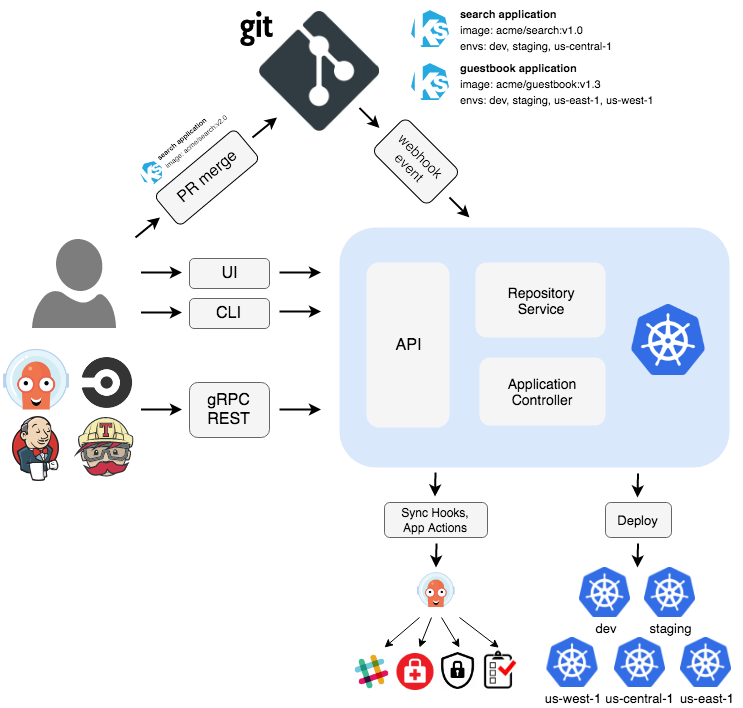
\includegraphics[scale=0.4]{Pictures/CI-CD/argocd_architecture.png}
\captionsetup{margin=1.5cm,format=hang,justification=justified}
\caption[]{Architecture de l'environnement Argo \newline}
\end{figure}


\begin{figure}[H]
\renewcommand{\figurename}{Graphique}
\hspace{-2.5cm}\includegraphics[scale=0.5,trim={0 0 5cm 0},clip]{Pictures/CI-CD/Onyxia-argo.PNG}
\captionsetup{margin=1.5cm,format=hang,justification=justified}
\caption[]{Deploiement de Onyxia dans argo \newline}
\end{figure}
 
\begin{interrupt}
\paragraph{Les avantages du GitOps}
\begin{itemize}
    \item Le répertoire Git contient l'historique des modifications. Cela permet de voir comment l'infrastructure a évoluée. Les messages de commits s'ajoutent à la documentation déjà existante. De plus, cela permet de voir le déploiement comme du code. On peut donc désormais pratiquer les techniques de "pair programming" ou d'"extreme programming" qui ne peuvent être que bénéfique. En effet, ces pratiques apportent beaucoup sur la qualité de code et de partage de connaissance sur le projet.
    \item Les tickets kanboard n'ont plus de raison d'être et sont remplacés par des merges requests. La pull request explique les besoins et le validateur review la merge request et la valide. On a donc deux avantages : : une réduction des erreurs humaines et un partage de connaissance.
    \item Revenir en arrière suite à un déploiement, revient simplement à faire un git revert sur le dernier commit.
    \item Comme tous les changements passent par Git, les modifications sont auditables. De plus, avec le  modèle en pull, seul l’opérateur a le droit de déployer dans le cluster. Il n'y a donc plus besoin de stocker les identifiants du cluster dans Git pour le CI, ce qui augmente la sécurité du cluster.
\end{itemize}
\end{interrupt}


\chapterimage{/chapter-image/onyxia.png}
\chapter{Onyxia: des services en self-déploiement}
\vspace{-2cm}

\section{Fonctionnement d'Onyxia}
Onyxia est une application composée de 2 parties : Onyxia-api (une API java pour les traitements) et Onyxia-ui (une interface React pour interagir avec l'utilisateur). Onyxia est une application que l'on qualifie de cloud-native, elle respecte l'architecture micro-service, elle repose sur une API rest et elle s'exécute dans des conteneurs. Elle est aussi stateless\footnote{} et scalable\footnote{}.\\

\begin{wrapfigure}[20]{r}{0.5\textwidth}
    \vspace{-1cm}
    \renewcommand{\figurename}{Diagramme}
    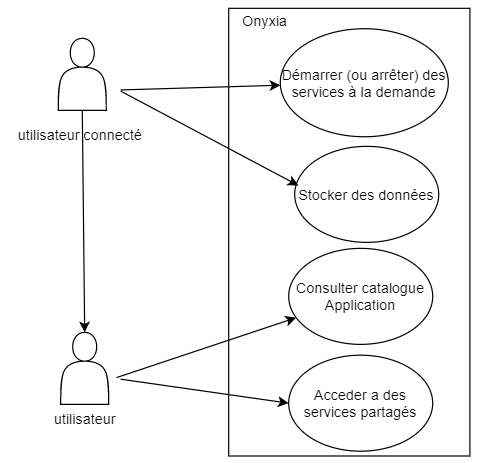
\includegraphics[scale=0.7]{Pictures/onyxia/onyxia-cu.PNG}
    \caption[]{Diagramme de cas d'utilisation \newline}
\end{wrapfigure}

L'application permet à l'utilisateur non connecté d'accéder aux autres services proposés par l'innovation on citera notamment rocket-chat (messagerie instantanée), minIO (stockage), Gitlab, ... L'utilisateur non connecté peut également consulter les catalogues de services à la demandes que propose Onyxia. L'utilisateur connecté peut lancer un service à la demande, le configurer (par exemple lancer un vs-code préconfigurer pour faire du python). Cet utilisateur peut aussi stocker des données. Onyxia s'interface avec minIO pour y uploader les données de l'utilisateur.\\

La spécifité d'Onyxia est que l'ensemble des services à la demande qu'elle offre aux utilisateurs sont pré-configurés. Aucune configuration d'un point de vue technique n'est demandé à l'utilisateur. En effet, lors d'un déploiement Onyxia agrège 3 sources de données afin de configurer le service de l'utilisateur. \\

Onyxia-ui fourni des données provenant de deux sources : les données saisies par l'utilisateur (la mémoire ou le nombre de cpu alloué pour le service) et les données permettant l'accès aux autres services (la configuration git, vault et/ou minIO). Onyxia-api apporte, elle aussi, des informations comme le choix de l'url du futur service déployé\footnote{Si 2 utilisateurs possédait chacun un service différents mais avec le même url, les utilisateurs aurait tantôt accès à un service tantôt a l'autre de manière totalement aléatoire}.\\

Ensuite, Onyxia dispose pour chaque service d'un template qui le décrit. Ce template est alors rempli à l'aide des valeurs précédemment crée.\\

Enfin dans un dernier temps, si le lancement du service n'est pas une simulation \footnote{En effet onyxia permet a ces utilisateurs de lancer une application en mode dry-run (i.e en mode simulation) pour permettre au personne les plus motivées de découvrir la configuration de leurs services}, Onyxia envoie le déploiement a l'orchestrateur, qui va désormais s'occuper de déployer, et de maintenir en vie le service jusqu'à son extinction.

\begin{figure}[H]
\renewcommand{\figurename}{Diagramme}
\hspace{-1cm}
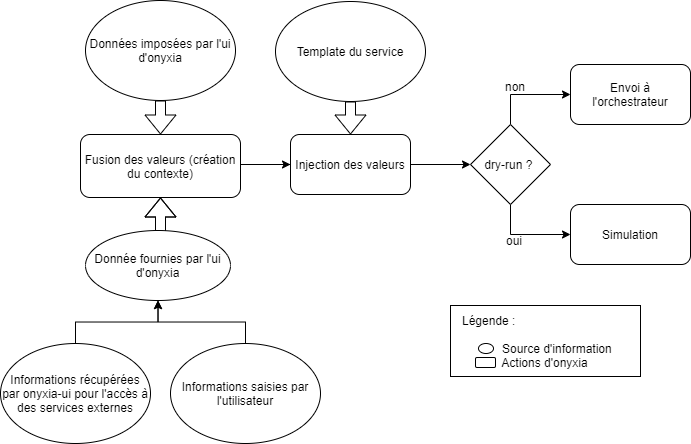
\includegraphics[scale=0.7]{Pictures/onyxia/onyxia-simplification.png}
\captionsetup{margin=1.5cm,format=hang,justification=justified}
\caption[]{Processus de déploiement d'un service par Onyxia \newline}
\end{figure}

Ce workflow est pour le moment uniquement réalisable avec marathon. Au cours de cette partie nous verrons ce que Kubernetes implique comme modification dans les 3 phases suivantes:
\begin{itemize}
    \item Phase 1 : Lecture et affichage des catalogues
    \item Phase 2 : Lancer un service et y ajouter la configuration.
    \item Phase 3 : Récupérer mes services, accèder à leurs configurations, et pouvoir les arrêter.
\end{itemize}


\section{Onyxia : Marathon et/ou Kubernetes ?}
Nous ne traiterons pas des solutions techniques mises en place (car elles n'ont pas grand intérêt) mais plutôt des points commun entre les 2 solutions et des difficultés rencontrées, au cours de l'implémentation de kubernetes dans onyxia. Le but étant au final de voir quelle solution semble être le plus utile pour la mise en place de service en mode self-déploiement.\\
Nous avons choisi que dans le cadre de kubernetes l'outil Helm pour être l'équivalent de Universe.
\subsection{Phase 1: Afficher des catalogues}
\subsubsection{Points commun et différences}
Au cours de cette première partie nous allons comparé le format Universe et le format Helm dans le but d'en extraire des informations communes au 2 formats de templating. Si l'on compare la description du Universe.json \footnote{\url{https://inseefrlab.github.io/Universe-Datascience/universe.json}} avec celle du index.yaml du répertoire Helm \footnote{\url{https://inseefrlab.github.io/helm-charts-datascience/index.yaml}}, on remarque que les deux sont a peu de chose prêt composé d'une liste de paquets\footnote{L'universe n'est constitué que d'un tableau de paquets, alors que le index.yaml contient en plus la date de génération du fichier + la version de l'API kubernetes avec laquelle ce helm repo est compatible}. \\ 

\begin{wrapfigure}[20]{r}{0.4\textwidth}
\renewcommand{\figurename}{Tableau}
\begin{tabular}{@{}l l@{}}
\toprule
Universe package                              & Helm package                                  \\ \midrule
    \begin{tabular}[c]{@{}l@{}}
	 \textcolor{green}{name} \\
     \textcolor{green}{description} \\
	 \textcolor{green}{version} \\
    \textcolor{blue}{marathon}\\
    \textcolor{blue}{config}\\
    packagingVersion \\
    scm\\
    maintener \\
    website \\
    framework
    tags\\
    preInstallNotes\\
    postInstallNotes\\
    postUninstallNotes\\
    selected\\
    lastUpdated\\
    releaseVersion\\
    resource\\
    \end{tabular} & 
    \begin{tabular}[]{@{}l@{}}
	 \textcolor{green}{name} \\
	 \textcolor{green}{description} \\
	 \textcolor{green}{version} \\
	 \textcolor{red}{urls} \\
	 apiVersion \\
	 appVersion \\
	 created \\
	 digest \\
	 engine \\
	 home \\
	 icon \\
	 keywords \\ 
	 sources \\
    additionalProperties \\ \\   \\   \\
    \end{tabular} \\ \bottomrule
\end{tabular}
\caption[]{Liste des attributs des paquets Universe et Helm \newline}
\end{wrapfigure}

Par la suite si on s'intéresse aux paquets, on a les informations ci-contre. En vert les informations que l'on retrouve dans les deux représentations. \\

Il y a cependant une nette différence au niveau des fichiers de configurations et des templates. En effet dans le cadre d'un paquet universe, le template ainsi que la configuration sont directement dans la description du package alors que pour le paquet Helm (Chart), le fichier de templating ainsi que la configuration sont dans un tar disponible sur l'url qui accompagne le paquet. \\

Pour avoir le même comportement (entre Helm et Universe), pour chaque Chart nous téléchargeons le chart auquel nous récupérons le fichier de configuration. Ainsi chaque paquet (Universe ou Helm), à au moins un nom, une description, une version, et un fichier de configuration. On a donc le diagramme de classe suivant :


\begin{figure}[H]\centering
\renewcommand{\figurename}{Diagramme}
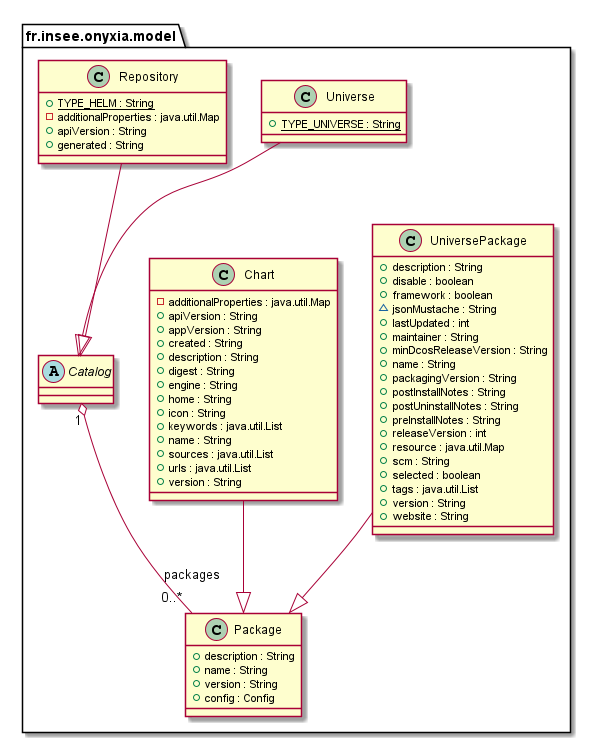
\includegraphics[scale=0.5]{Pictures/onyxia/testdiagram1.png}
\captionsetup{margin=1.5cm,format=hang,justification=justified}
\caption[]{Diagramme de classe des entitées catalogues + packages dans Onyxia \newline}
\end{figure}
\vspace{-2cm}
\begin{interrupt}
Un répertoire Helm ou Universe sont vu comme un catalogue. Chacun de ses catalogues sont composés de paquets qui peuvent-être soit des Charts (Helm) ou des UniversePackages (Universe). Un paquet est au moins caractérisé par un nom, une description, une version et un fichier de configuration auquel s'ajoute des informations appartenant a l'un ou l'autre des deux types de paquets.
\end{interrupt}

\begin{wrapfigure}[11]{l}{0.6\textwidth}
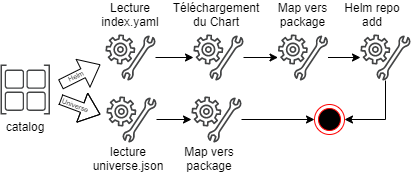
\includegraphics[scale=0.6]{Pictures/onyxia/workflow-catalog.png}
\caption{Workflow lecture et ajout de catalogue \newline}
\end{wrapfigure}
L'ensemble des catalogues proposé par Onyxia sont décrit dans un fichier json. Ce fichier comporte notamment le type du catalogue (Universe ou Helm) et l'url sur lequel se trouve le fichier décrivant le catalogue (respectivement le universe.json ou le index.yaml). Le workflow ci contre s'exécute alors périodiquement afin d'ajouter les différents paquets dans onyxia.

\subsubsection{Difficultés rencontrées}
Au cours de cette première partie la principale difficulté est venu des catalogues Helm. En effet, DC/OS propose une dépendances Maven permettant de wrapper le fichier universe.json vers des classes Java. Il n'existe cependant pas d'équivalent pour Helm. Il a donc fallu implémenter à la main le mapping de l'index.yaml vers Java. Il nous a également fallu exécuter des commandes Helm (notamment pour l'ajout du répertoire dans Helm). Je n'ai trouvé aucune dépendance Java qui le permettait. Il a donc fallu ajouter à Onyxia un module permettant d'interagir avec Helm par l'intermédiaire d'éxécution de ligne de commande depuis java, ce qui a aussi impliqué d'ajouter Helm et Kubernetes à l'image docker d'Onyxia.

\subsection{Phase 2: Lancer des services et les configurer}
\subsubsection{Points commun et différences}
Cette partie débute au moment ou l'utilisateur se retrouve sur la page de configuration de son service sur onyxia. Que le service proviennent d'un paquet Universe ou Helm, l'expérience utilisateur est la même mais l'implémentation diffère. En effet lors de la création d'un service on a le workflow \footnote{On ne fait pas apparaître ici comment Onyxia-ui récupère les informations techniques de l'utilisateur (Vault, Git, Minio)} suivant : 
\begin{figure}[H]\centering
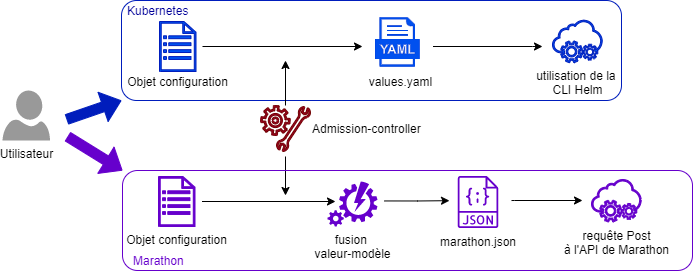
\includegraphics[scale=0.6]{Pictures/onyxia/publish-service.png}
\captionsetup{margin=1.5cm,format=hang,justification=justified}
\caption{Workflow du déploiement d'un service \newline}
\end{figure}
Dans le cas Helm ou Universe, Onyxia-api reçoit un objet de type Map<String,Object> (une liste de clé-valeur) contenant la configuration du service. Cependant certains paramètres reste à injecter: on trouve l'url, le nom du service, etc... c'est le rôles des admissions-controller.\\
Les admissions-controller parcourent l'ensemble de la Map contenant la configuration, et y ajoute la clé et la valeurs du paramètre qu'ils auront générés. Ainsi dans le cas Universe et Helm, on ne possède pas les mêmes admissions-controller : \begin{itemize}
    \item Pour Universe, on a un admission-controller qui va gérer le nom du service. En effet marathon ne possède pas la notion de namespace, mais plutôt de dossier \footnote{L'innovation à fait le choix que les services demandés par une personne se situe dans l'arborescence suivante users/idep/} et ce dossier est déterminé en fonction de l'id du service. On doit donc injecter User-idep- dans le nom du service. Par ailleurs un dossier ne peut pas contenir 2 noms de services identiques, il faut donc randomiser le nom du service, l'admission controller ajoute un nombre aléatoire à la suite du nom du service (pour vs-code on aurait par exemple users/idep/vscode-1234). Enfin un autre admission-controller genère l'URL d'accès au service en fonction de l'idep du nom de service, du domaine sur lequel Onyxia est configuré pour déployer.\footnote{Pour éviter les doublons ce générateur d'url ajoute un nombre aléatoire à l'URL}
    \item De son coté Helm ne nécessite qu'un seul admission-controller celui de l'URL. Il repose sur le même générateur que Marathon, mais cela ne se traduit pas par la même clé dans la map des valeurs (normal puisque Helm et universe possède une syntaxe différente).
\end{itemize}

\begin{interrupt}
\paragraph{Remarques:}
 Dans le cas de Helm, on n'a pas d'admission-controller qui injecte un id de service et/ou l'idep de la personne dans les values, car ces derniers s'injecte au moment de l'exécution de la commande helm par le biais des options (-n pour le namespace et --generate-name pour l'id). \\
 Toujours dans le cas de Helm, la détermination du namespace de l'utilisateur entraîne sa création par Onyxia si ce dernier n'existe pas.
\end{interrupt}
Ensuite dans le cas de Universe, le template du service est rempli (mustaché) à l'aide de la map contenant la configuration \footnote{C'est l'équivalent de jq en ligne de commande}. Une fois cette opération on a donc un fichier marathon.json classique remplie à l'aide des valeurs précédentes. Si il s'agissait d'un lancement de type dry-run alors on renvoie à l'utilisateur ce fichier, sinon on envoie ce fichier directement sur l'endpoint v2/deployments de Marathon.\\

Pour Helm, on traduit la map contenant la configuration en un fichier de type values.yaml et on éxécute la ligne de commande \texttt{Helm apply my-app -f my-values -n namespace} avec ou sans l'option \texttt{--dry-run} en fonction de la demande de l'utilisateur. C'est donc Helm qui se charge de la récupération du template, de l'injection des valeurs ainsi que de la communication a Kubernetes du déploiement.

\subsubsection{Difficultés rencontrées}
Au cours de cette partie, les difficultés sont venues de la partie Helm. En effet DC/OS propose un client Marathon (pour dialoguer directement avec marathon), et il existe une dépendance maven facilitant le remplissage des template \footnote{Lien vers le projet: \url{https://github.com/spullara/mustache.java}}.\\
Pour pouvoir installer une application en utilisant Helm, il fallait d'abord que l'utilisateur possède un namespace dans Kubernetes. Pour cela nous avons du autoriser onyxia à créer des namespaces et faire en sorte qu'Onyxia puisse dialoguer avec Kubernetes. Pour cela nous avons utiliser la dépendance maven fabric8.kubernetes-client, qui fournit une bibliothèque complète permettant de dialoguer avec Kubernetes depuis java. \\
Enfin, afin qu'Onyxia puisse créer des namespaces il fallait lui donner des droits dans le cluster Kubernetes. Initialement, nous voulions lui donner les droits cluster-admin uniquement sur l'ensemble des namespaces commençant par "user-...",les namespaces qu'onyxia devait gérer, mais cela n'est pas possible actuellement\footnote{issue disponible ici : \url{https://github.com/kubernetes/kubernetes/issues/56582} fermée mais non résolue}, nous lui avons donc donné le rôle cluster-admin (ce n'est pas idéal puisque onyxia pourrait donc interférer sur des namespaces qui ne lui sont pas dédié).

\subsection{Phase 3: Récupérer des services, leurs configurations et les arrêter}
Cette partie a sûrement été la plus facile d'un point de vue technique. La principale différence réside dans le fait que pour les paquets universes l'ensemble des actions se font par l'intermédiaire du client marathon  et les résultats sont mappés à l'aide des classes fournies par DC/OS. Alors que dans le cas de Helm l'ensemble des actions se font depuis ce dernier et aucune implémentation de mappeur n'existe, il a donc fallu à chaque fois le faire à la main.\\

\begin{table}[H]
\hspace{-1.5cm}
\begin{tabular}{@{}lll@{}}
\toprule
                                                                                     & Universe             & Helm                                                                                                                             \\ \midrule
Arrêter un service                                                                   & requête sur endpoint & helm rm nomRelease -n namespace                                                                                                  \\
\begin{tabular}[c]{@{}l@{}}Lister mes services + \\ Détail d'un service\end{tabular} & requête sur endpoint & \begin{tabular}[c]{@{}l@{}}helm ls -n namespace + \\ helm get manifest nomRelease -n namespace pour chaque release\end{tabular} \\ \bottomrule
\end{tabular}
\end{table}
Pour Helm, chaque requête sur Onyxia-api pour lister mes requêtes résulte en fait en n+1 requêtes. En effet on a d'abord une première requête pour lister le nom des services qui s'exécutent, et ensuite pour récupérer les détails, il faut faire une requête par services ce qui conduit au final à n+1 requêtes (en comparaison, il suffit d'une seule requête pour les paquets Universes). \\

Par ailleurs le comportement de helm n'est pas le même que marathon lorsqu'on stoppe un service. En effet marathon distingue un service arrêté d'un service supprimé, ce n'est pas le cas de Helm. Un service helm que l'on arrêtera sera perdu (il faudra repasser par l'étape de création pour en avoir un nouveau) alors qu'un service universe déployé dans marathon pourra être redémarré.

\section{Quel intêret pour l'Insee ? Pour la statistique publique ?}
La migration d'Onyxia vers Kubernetes a permis à l'Insee de ne plus être dépendante de DC/OS. En effet nous sommes désormais capable de monter une deuxième plateforme de l'innovation sans ces outils. Cette migration à également permis de moderniser, de rendre open-source et rajouter des fonctionalités à Onyxia : le support de kubernetes, mais aussi le cloudshell \footnote{Un shell directement accessible dans Onyxia et permettant de dialoguer directement avec le cluster et/ou les différences tel que git, minio, vault }, ou encore le multi-régions \footnote{Initialement, onyxia ne pouvait déployer que dans un seul orchestrateur. Désormais l'utilisateur peut déployer des applications dans plusieurs lieux qu'il peut choisir depuis Onyxia.}. Ces travaux permettront également d'améliorer sa disponibilité puisque plusieurs centre Insee peuvent désormais facilement déployer et héberger leur Onyxia.\\

Cette migration permet également de proposer aux autres établissements du ministères des finances une solution pour se créer un cloud spécialisé dans les outils et techniques de traitement de données, à l’état de l’art et accessible à un public varié 100\% gratuite et opensource. A une époque ou les établissements privés semblent prendre petit à petit le pas sur les missions des établissements publics, l'existence d'une telle solution ne peut-être que bénéfique. Cette plateforme permettant de rendre les techniques modernes plus accessibles et de mutualiser les efforts pour répondre aux défis actuels de la statistique publique.



\chapterimage{chapter-image/autre-01.jpg} 
\chapter{Autre}
\vspace{-2cm}
Dans cette partie nous aborderons divers point qui différencie Kubernetes et Marathon de DC/OS. Nous aborderons notament la partie interfaçage avec le cloud et la partie outils de debuggage.

\section{Interfaçage avec le cloud}
Lorsqu'on choisit son orchestrateur de conteneur, on tient forcement compte de la facilité de déploiement de ce dernier. En effet, en général on veut que notre infrastructure soit déployable facilement, rapidement, et sans faire face une très grande complexité de configuration.   
\subsection{Rappels : Paas, Saas, Iaas}
Avant de parler de comment déployer notre orchestrateur dans le cloud revenons sur l. Le cloud permet d’entreposer sur des serveurs à distance des logiciels et des données. Les fournisseurs cloud proposent différentes types de services clouds. On retrouve:
\begin{itemize}
    \item Iaas (infrastructure as a service) : Dans ce type d'offre l'utilisateur doit configurer l'ensemble de l'infrastructure informatique. Cela concerne notamment les serveurs, le réseaux, le stockage de donnée, ou encore la solution de virtualisation choisie. Cette offre cloud demande à l'administrateur de forte compétence tantôt sur les systèmes d'exploitations, les données ou encore sur le réseau. L'IAAS permet de dématérialiser l'ensemble de l'infrastructure matérielle.
    \item Paas (plateform as a service): Dans cette solutions, le fournisseur propose l'ensemble des solutions IAAS auquelle il ajoute également la configuration des middleware : Système d'exploitation, configuration réseau etc... Aucune configuration technique n'est requise.
    \item Saas (Software as a Service): Une solution SAAS regroupe l'ensemble des services SAAS et IAAS auxquelle s'ajoute l'installation, la maintenance et la gestion des applications. Cette solution permet la simple utilisation des services et ne nécessite aucune expertise technique ou informatique. Par exemple gmail est une application SAAS
\end{itemize}


\begin{figure}[H]\centering
\renewcommand{\figurename}{Graphique}
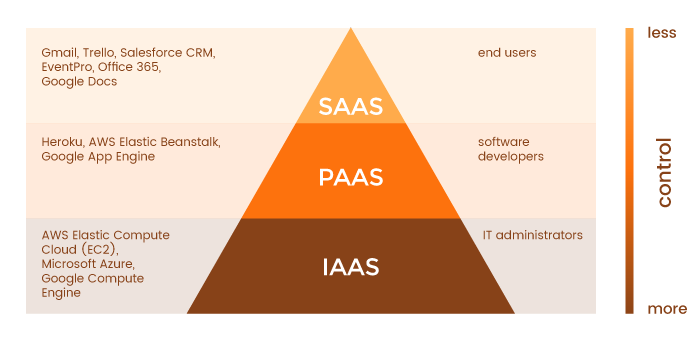
\includegraphics[scale=0.6]{Pictures/Comparaison/cloud/difference-cloud.png}
\captionsetup{margin=1.5cm,format=hang,justification=justified}
\caption[]{Différence Iaas, Saas, Paas \newline}
\end{figure}

Dans le cas du développeur qui veut pouvoir déployer rapidement ces applications, il est intéressant d'avoir accès à une offre Saas.

\subsection{Comparaison offre Cloud Marathon et Kubernetes}
De part son succès de nombreux provider cloud proposent une offre Kubernetes: parmi eux on peut citer Microsoft Azure, Amazon EKS (Amazon Elastic Kubernetes Service), ou encore GKE (Google Kubernetes Engine), etc... Ces offres proposent de créer des clusters Kubernetes en quelques minutes seulement. Par exemple, il suffit de quelque clics (choix du nombre et du type des workers nodes, localisation du cluster et la version de Kubernetes) pour lancer un cluster Kubernetes dans GKE. Ici on parle d'offre Saas (ou clés en main), en effet une fois le cluster créé, le développeur peut directement y déployer ses applications.\\

Pour le développeur qui veut tester Kubernetes sans avoir a lancer un cluster dans le cloud de nombreuse solutions existe pour lancer un cluster Kubernetes en local: minikube avec virtualbox, k3s avec docker. Ces offres proposent des clusters Kubernetes déja configuré avec un seul worker node, permettant au développeur de tester facilement les possibilités que peut offrir Kubernetes.\\

Kubernetes centralise l'ensemble des providers cloud qui fournissent des solutions ici : \url{https://Kubernetes.io/fr/docs/setup/pick-right-solution/}. \\

A l'inverse, pour Marathon il n'existe pas de solutions Saas. Le seul moyen de lancer un cluster Mesos avec Marathon dans le cloud est de souscrire a une offre Iaas. Par la suite, l'utilisateur doit configurer ses machines, en y installant l'ensemble des briques Mesos ou en utilisant l'outils d'installation DC/OS. De la même façon, il est impossible de lancer un cluster Mesos avec Marathon en local sans devoir configurer l'ensemble de la sphère Mesos. Cette différence s'explique notamment par le fait que les utilisateurs de Mesos, n'utilise par ce dernier uniquement pour avoir Marathon comme Scheduler. Le provider cloud n'a donc aucun intêret à proposer une offre packagée.\\

Par ailleurs de nombreux fournisseurs cloud sont désormais pris en charge par Terraform. Terraform est un outils qui permet d'automatiser la création de ressources dans le cloud (Terraform est au cloud ce que Puppet est aux VMs). Terraform est donc un bon outils pour automatiser la création d'un cluster Mesos avec Marathon ou Kubernetes. Pour plus d'information sur Terraform se rendre à l'annexe X. Enfin l'outil Rancher permet de créer rapidement des clusters kubernetes au sein de VM située dans le cloud ou dans un datacenter \footnote{\url{https://enix.io/fr/blog/rancher-2-trois-methodes-d-installation/}}.

\section{Les outils de débuggage}
Un autre point qui intéresse le développeur ce sont les outils de développement qui accompagne chaque orchestrateur. En effet un orchestrateur est attractif, si il est simple de développer, de débugger, de surveiller ses applications avec ce dernier.\\

Avec Marathon les outils mis à la disposition du développeur sont peu nombreux. En effet la ligne de commande DC/OS permet uniquement de déployer une application. l'interface admin de Mesos permet de suivre l'état du cluster, consommation de chaque node, gestion des alertes etc... Par l'intermédiaire de l'UI (ou de la cli) de Marathon le développeur peut consulter les logs d'exécution de ses Pods. La cli Mesos permet également d'exécuter directement du code dans un conteneur, ce qui peut être utile pour debugger. Mais encore une fois il faut configurer la cli de Mesos ce qui n'est pas évident et la gestion des droits n'est pas aisée. C'est d'ailleurs pour cette raison que l'innovation possède 2 Marathon. Le premier est dédié au développeur dans le cadre de l'intégration continue, le deuxième était réservé au déploiement de gitlab, rocketchat, etc... \\

Kubernetes propose lui aussi toute ces fonctionnalités. L'équivalent de l'interface administrateur est le Kubernetes dashboard, mais puisque les identifiants de connexions sont des tokens Kubernetes, le dashboard permet également la restriction de ressource et/ou de namespace. La cli kubectl apporte de nombreuses autres possibilités, comme par exemple la possibilité de "port-forward" un Pod. Cela permet au développeur d'exposer son Pod directement en localhost, ça peut permettre de mieux cerner les problèmes : problème au niveau du Pod, ou au niveau de l'ingress. La cli kubectl permet également de faire des rollback sur nos déploiements. Par ailleurs, de nombreuse extensions existe, notamment l'extension vscode Kubernetes qui detecte automatiquement la configuration Kubernetes présente sur notre poste.  Cela permet notament de rassembler l'ensemble des outils du developpeur au même endroit. Cette extension permet également de générer des squelettes de deployments, services, ingress. Il existe aussi l'outil lens qui est un ide pour kubernetes \footnote{\url{
https://github.com/lensapp/lens}}.

\part{Conclusion et annexes}
\chapterimage{/chapter-image/conclusion.png}
\chapter{Conclusion}

\appendix

\chapterimage{/chapter-image/deployer.png}
\chapter{Déployer une Application}
\label{}
\vspace{-2cm}
\section*{Marathon: le endpoint /v2/deployments}
Il faut savoir que un déploiement dans marathon ce fait par l'intermédiaire d'un fichier JSON décrivant l'état souhaité du déploiement. Nous allons partir de l'exemple ci dessus qui permet de déployer dans marathon un vs-code permettant de faire du python.
\begin{minted}[mathescape,
               linenos,
               numbersep=5pt,
               gobble=2,
               frame=lines,
               framesep=2mm]{csharp}
{
  "id": "/users/ystfg5/vscode-6300374061626994050",
  "container": {
    "type": "DOCKER",
    "docker": {
      "image": "inseefrlab/vscode-python",
      "forcePullImage": false,
      "privileged": false,
      "parameters": []
    },
    "volumes": [],
    "portMappings": [
      {
        "containerPort": 8080,
        "hostPort": 0,
        "protocol": "tcp",
        "servicePort": 10126
      }
    ]
  },
  "env": {
    "PASSWORD": "changeme",
    "PORT": "8080"
  },
  "labels": {
    "HAPROXY_0_REDIRECT_TO_HTTPS": "true",
    "HAPROXY_GROUP": "external",
    "HAPROXY_0_ENABLED": "true",
    "MARATHON_SINGLE_INSTANCE_APP": "true",
    "HAPROXY_0_VHOST": "ystfg5-vscode-6300374061626994050.lab.sspcloud.fr"
  },
  "cpus": 0.1,
  "disk": 0,
  "instances": 1,
  "maxLaunchDelaySeconds": 300,
  "mem": 2048,
  "gpus": 0,
  "networks": [
    {
      "mode": "container/bridge"
    }
  ]
}

\end{minted}
Si on découpe le contrat ci dessus on a les parties suivantes : 
\begin{itemize}
    \item id :
    \item container
    \item env
    \item labels
    \item volumes
    \item networks
    \item instance 
\end{itemize}
\section*{Kubernetes : le trio ingress.yaml, service.yaml, deploiement.yaml}

Tout d'abord,il faut savoir que les déploiements Kubernetes sont, en général, configurés dans des fichiers .yaml (équivalent de JSON). Pour ce Hello world, nous allons tenter de déployer un serveur tomcat. Nous allons avoir besoin de 3 fichiers (on peut néanmoins les regrouper en 1 seul fichier mais pour plus de lisibilité nous les séparerons) 

\subsection*{Deployment.yaml}
Un deployment correspond à l'orchestration de Pods. Le deployment s'assure que l'application tourne bien, avec un nombre d'instances correspondant au nombre demandé. Si l'on regarde le fichier deployment.yaml : 
\usemintedstyle{colorful}
\begin{minted}[mathescape,
               linenos,
               numbersep=5pt,
               gobble=2,
               frame=lines,
               framesep=2mm]{csharp}
    apiVersion: extensions/v1beta1
    kind: Deployment
    metadata:
        name: hello
    spec:
    replicas: 2
    selector:
    matchLabels:
      app: hello
    template:
        metadata:
            labels:
                app: hello
    spec:
      containers:
        - name: hello
          image: tomcat:9.0.29
\end{minted}

On retrouve 2 informations intéressantes : 
\begin{itemize}
    \item le champ replicas qui corresponds au nombre de conteneurs que l'on va lancer dans le cluster. On parle alors de scalabilité horizontale. 
    \item le champ image qui corresponds à l'image docker que nous allons déployer dans Kubernetes.
    \item les autres champs sont essentiellement des champs qui serviront a Kubernetes comme identifiant.
\end{itemize}
Executons le fichier que l'on vient de créer, pour cela nous utiliserons la ligne de commande :
\usemintedstyle{colorful}
\begin{minted}[mathescape,
               linenos,
               numbersep=5pt,
               gobble=2,
               frame=lines,
               framesep=2mm]{python}
               kubectl apply -f deployment.yaml
\end{minted}
Notre Pod est désormais deployé, mais il tourne dans le cluster mais impossible d'accéder à ce déploiement. 
\subsection*{Service.yaml}
Chaque Pod possède une adresse IP qui lui est propre, on pourrait donc imaginer donné accès a cette adresse ip aux utilisateurs. Mais lorsqu'on diffuse une application, on expose un service qui sera rendu par plusieurs Pod, donner l'ip du Pod aux utilisateurs n'est donc pas le meilleur moyen. De plus, tous les clients de l'application (en particulier les autres microservices du cluster) n'ont pas à savoir où sont les Pods précisemment. \\
Par ailleurs, Kubernetes propose et impose un découplage fort entre le service rendu et l'application qui le rend. \\ 

Le concept de service va donc nous aider. Un service permet d'exposer un port du conteneur (ici, le port 8080 de notre tomcat) à l'intérieur du cluster (on ne parle pas encore d'exposition vers l'extérieur, ça viendra avec le concept suivant). \\
Le contrat du service est le suivant : 
\usemintedstyle{colorful}
\begin{minted}[mathescape,
               linenos,
               numbersep=5pt,
               gobble=2,
               frame=lines,
               framesep=2mm]{csharp}
    apiVersion: v1
    kind: Service
    metadata:
        name: hello
    spec:
        ports:
            - name: http
              targetPort: 8080
              port: 80
    selector:
        app: hello
\end{minted}
Les infos les plus importantes sont : 
\begin{itemize}
    \item name : le nom donné au port exposé (sera utilisé plus tard)
    \item targetPort : le port du conteneur (pour tomcat : 8080)
    \item port : le port sur le service (non utilisé dans ce tutorial)
\end{itemize}

Après execution du service.yaml (avec kubetcl apply) le service est bien en place, notre tomcat est maintenant accessible mais ... uniquement depuis l'intérieur du cluster. (pour s'en convaincre \textit{kubectl get services} noter l'adresse ip,puis lancer  \textit{kubectl run -i --tty busybox --image=busybox --restart=Never -- sh } qui permet de lancer un deployment en mode interactif et nous donne accès a son shell, executer ensuite curl adresse-ip:80 notre service répond)

\subsection*{Ingress.yaml}
L'ingress est le fichier qui va nous permettre d'exposer notre service a l'extérieur du cluster. Un ingress correspond à un point d'entrée dans le cluster. Ca va nous permettre d'exposer notre service en dehors du cluster ! C'est globalement équivalent au travail classique d'un reverse-proxy.

\usemintedstyle{colorful}
\begin{minted}[mathescape,
               linenos,
               numbersep=5pt,
               gobble=2,
               frame=lines,
               framesep=2mm]{csharp}
    apiVersion: extensions/v1beta1
    kind: Ingress
    metadata:
      name: hello
      annotations:
        Kubernetes.io/ingress.class: nginx
    spec:
        tls:
            - hosts:
                - amodifier.portail.innovation.insee.eu
    rules:
        - host: amodifier.portail.innovation.insee.eu
            http:
            paths:
                - path: /
                backend:
                    serviceName: hello
                    servicePort: http
\end{minted}
Quelques informations importantes :

\begin{itemize}
    \item \texttt{annotations: Kubernetes.io/ingress.class: nginx} : une indication pour dire le reverse-proxy à utiliser. Sur le cluster innovation, il s'agit de nginx (mais sur d'autres clusters, on pourrait trouver du traefik, du ha\_proxy ...).
    \item \texttt{rules: - host: amodifier.portail.innovation.insee.eu}: Le nom de domaine à utiliser pour l'entrée. Sur le cluster innovation, toutes les URL doivent être de la forme x.portail.innovation.insee.eu
    \item \texttt{tls: - hosts: - amodifier.portail.innovation.insee.eu}: L'activation du TLS (le s de https) pour notre domaine. L'application sera automatiquement servie en HTTPS avec un certificat ajouté par le reverse proxy
\end{itemize}

Désormais en se rendant sur l'url : \texttt{amodifier.portail.innovation.insee.eu} on accède à notre application. Ici nous venons de déployer une application simple et nous avons déja 3 fichiers de configurations (nous n'avons pas ici d'injection de variables d'environnement, ou de création de namespace,etc...).\newline


\section*{Migrer facilement des tâches Marathon vers des jobs Kubernetes}
Pour les applications possédant un contrat Marathon fixe et qui est exécuté chaque jour, il pourrait être intéressant de posséder un convertisseur de contrat Marathon vers des contrats Kubernetes. Un projet regroupant ce type de fonctionnalité existe déjà : \url{https://github.com/micahhausler/container-transform} développé par Micah Hausler un développeur travaillant chez AWS. Cependant, ce projet n'est plus maintenu depuis au moins 3 ans, l'évolution de Kubernetes est telle que ce projet est dépassé (de nouveaux objets sont apparus dans Kubernetes depuis). Nous avons donc créé un convertisseur de contrat Marathon vers Kubernetes: \url{https://github.com/InseeFrLab/marathon-to-Kubernetes}. Ce projet Java openSource s'appuie sur deux librairies: \begin{itemize}
    \item mesosphere/marathon-client : une librairie permettant de communiquer avec l'API de Marathon. Elle nous permet de convertir nos fichiers "marathon.json" en objets Marathon.
    \item io.fabric8/Kubernetes-client: une librairie permettant de communiquer avec l'api-server de Kubernetes. Elle permet notamment la création d'objet Kubernetes.\newline 
\end{itemize}

Actuellement, l'application est capable de convertir un contrat Marathon contenant une ou plusieurs applications, en ajoutant les limites de ressources, les ingress, et en injectant les configurations nécessaires. Cependant, deux fonctionnalités restent à développer. En effet, les contrats Marathon disposent d'une partie fetch qui permet notamment de télécharger des ressources et les place dans la "sandbox", un dossier accessible par tous les conteneurs du contrat. Cette notion de fetch n'existe pas directement dans Kubernetes, il faut créer des init-containers, des conteneurs qui s'exécuteront avant notre conteneur contenant l'application. Une autre fonctionnalité est le fait de pouvoir convertir un groupe d'applications comme par exemple la brique ELK (ElasticSearch, Logstash, Kibana).\newline

Le but originel de ce projet était de pouvoir convertir un contrat Marathon en contrat Kubernetes à la volée dans Onyxia, afin de pouvoir migrer rapidement des déploiement marathon vers Kubernetes afin de tester si le cluster Kubernetes interne supportait ou non la charge. Nous n'avons donc pas poussé l'implémentation plus loin, cependant ce projet est utilisable en l'état.
\begin{figure}[H]\centering
\renewcommand{\figurename}{Tableau}
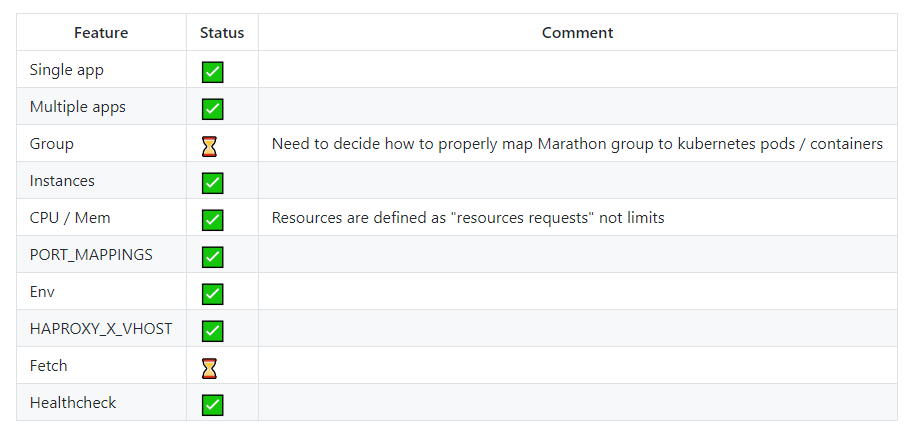
\includegraphics[scale=0.6]{Pictures/CI-CD/marathon-to-kub.PNG}
\captionsetup{margin=1.5cm,format=hang,justification=justified}
\caption[]{Recapitulatif des fonctionnalités prisent en charge par l'application \newline}
\end{figure}




\chapterimage{chapter-image/security-01.jpg} 
\chapter{Kubernetes et sécurité} 
\vspace{-2cm}
(plutot en annexe)
ajout de l'identification keycloak sur l'api
onykub on ne peut lancer des deploiments uniquement dans son namespace d'une application au sein de son namespace

\section*{Reverse proxifier l'api-server}

\section*{Open Policy Agent (OPA)}

\chapter{Kubernetes, GKE, et terraform}
\section*{Création d'un compte gcloud à l'INSEE}
Afin de pouvoir travailler sur Kubernetes à la fois à l'Insee et à la fois en extérieur de l'Insee j'ai d'abord utilisé minikube, mais cette solutions offrait vite ses limites : environnement avec un seul node qui n'est pas du tout représentatif d'un environnement standard Kubernetes, je voulais par ailleurs conservé les configurations que j'avais pu faire sur mon cluster Kubernetes, j'ai donc choisi de me creer un cluster Kubernetes dans le cloud de google. Je vais ici expliquer ma démarche ainsi que les problèmes auxquels j'ai fait face et les solutions trouvé pour les contourner.\\

Tout d'abord je voulais avoir accès a mon cluster Kubernetes de n'importe où avec le moins de configurations possible sur le poste que j'utilisais (en effet les postes insee sont des windows et il n'est pas facile de travailler sur du Kubernetes depuis windows), j'ai donc crée dans le cloud google une instance de vm ubuntu (onglet Compute Engine)  qui me servirait de point d'entrée pour mon futur cluster Kubernetes et sur laquelle j'installerai tout les outils nécessaires.\\

J'ai ensuite ajouté dans l'onglet Metadata (toujours dans l'onglet Compute Engine) ma clé ssh. Cela me permet de me connecter simplement a cette vm depuis n'importe quel ordinateur dont la clès ssh a été ajoutée depuis l'onglet metadata : simplement en faisant \texttt{ssh ubuntu@ip-de-la-vm}. Cependant cette solution pose un problème :  Depuis l'INSEE les connexion ssh vers un nom de domaine sont autorisées mais celles vers une adresse ip sont bloquées par le proxy. Il fallait donc associer l'ip a une adresse http. J'ai donc du acheter un domaine internet : *.eneman.fr (je l'ai acheté chez ovh car c'était le moins cher) et redirigé toute les requetes sur ce domaine vers les dns google. Ce nom de domaine me servira également a exposer les futurs services que je déploierai dans Kubernetes\\

Enfin dans un dernier temps dans l'onglet Network services rubrique cloud dns de la console google cloud, j'ai rajouté une entrée \texttt{jumphole.eneman.fr} avec l'adresse ip de ma VM ubuntu pour redirigé toute connexion ssh sur cette machine. je pouvais désormais faire un  \texttt{ssh ubuntu@jumphole.eneman.fr}\\

Il fallait maintenant creer un cluster Kubernetes. J'ai donc essayé plusieurs moyen pour lancer mon cluster : 
\begin{itemize}
    \item depuis l'interface google cloud console onglet 
    \item depuis la ligne de commande gcloud
    \item A l'aide de terraform: terraform est un outil de création d'infrastructure as code. 
\end{itemize}

Nous allons donc lancer un cluster décrit par les paramètres ci dessus par les trois moyens cité précédemment: 
\begin{itemize}
    \item Le name donné au cluster
    \item le location-type : deux choix sont proposés: Zonal ou Regional. Sélectionner Regionnal permet de déployer des nodes Kubernetes dans chaques zones de la région, cela permet d'avoir une haute disponibilité, alors que zonal déploit dans une seule zone de la région choisie. Nous opterons pour un location-type zonal en europe-west3-b.
    \item la version de Kubernetes : nous choisirons ici le mode release-channel qui nous permettra de toujours choisir la version la plus récente proposée par google. (actuellement la 1.15.7)
    \item Enfin le type des machines, nous choisirons ici dans le cas des tests des machines de types g1-small.
\end{itemize}


\section*{Kubernetes à l'insee ?}
l'innovation c'est bien mais ...
Création d'un compte cloud.



\paragraph{Interface google cloud}
Afin de créer un cluster avec l'interface google cloud, il faut se rendre dans l'onglet Kubernetes, normalement, si on a aucun cluster déjà lancé, google propose d'en créé un. Les attributs necessaire pour obtenir un cluster Kubernetes sont les suivants :

Name -> location -> version de Kubernetes -> choix des noeuds -> valider
    Version to use the most up-to-date features
    Machine type to use a less expensive machine
    Boot disk size to use a less expensive boot disk
    Disable Autoscaling to avoid unnecessary cost
    Disable Stackdriver monitoring and logging to avoid unnecessary cost 

\paragraph{Gcloud}





\paragraph{lets encrypt}
le site exposé n'est pas reconnu par le proxy de l'insee qui n'aime pas les certificats auto-signés --> expliqué fonctionnement de lets encrypt --> certif valide 3 mois avec defi pour obtenir le certif


\chapterimage{/chapter-image/kubeapps.png}
\chapter{Kubeapps une alternative à Onyxia ?}
\vspace{-2cm}
Dans le monde de kubernetes, il existe des applications permettant de simplifier le déploiement de charts Helm. On citera notamment Kubeapps, Kubeapps est un chart helm qui permet de déployer une interface web permettant à son tour de déployer et de gérer des applications dans Kubernetes. Il permet d'ajouter des répertoires de chart Helm (aussi bien public que privé) et de les déployer dans le cluster. Kubeapps permet également de gèrer, monter les versions, et supprimer les applications que l'on a déployer dans le cluster. Cette application supporte également l'authentification oidc ce qui nous permettrai d'utiliser Keycloak comme provider d'authentification.

\begin{figure}[H]\centering
\renewcommand{\figurename}{Graphique}
\hspace{-1cm}
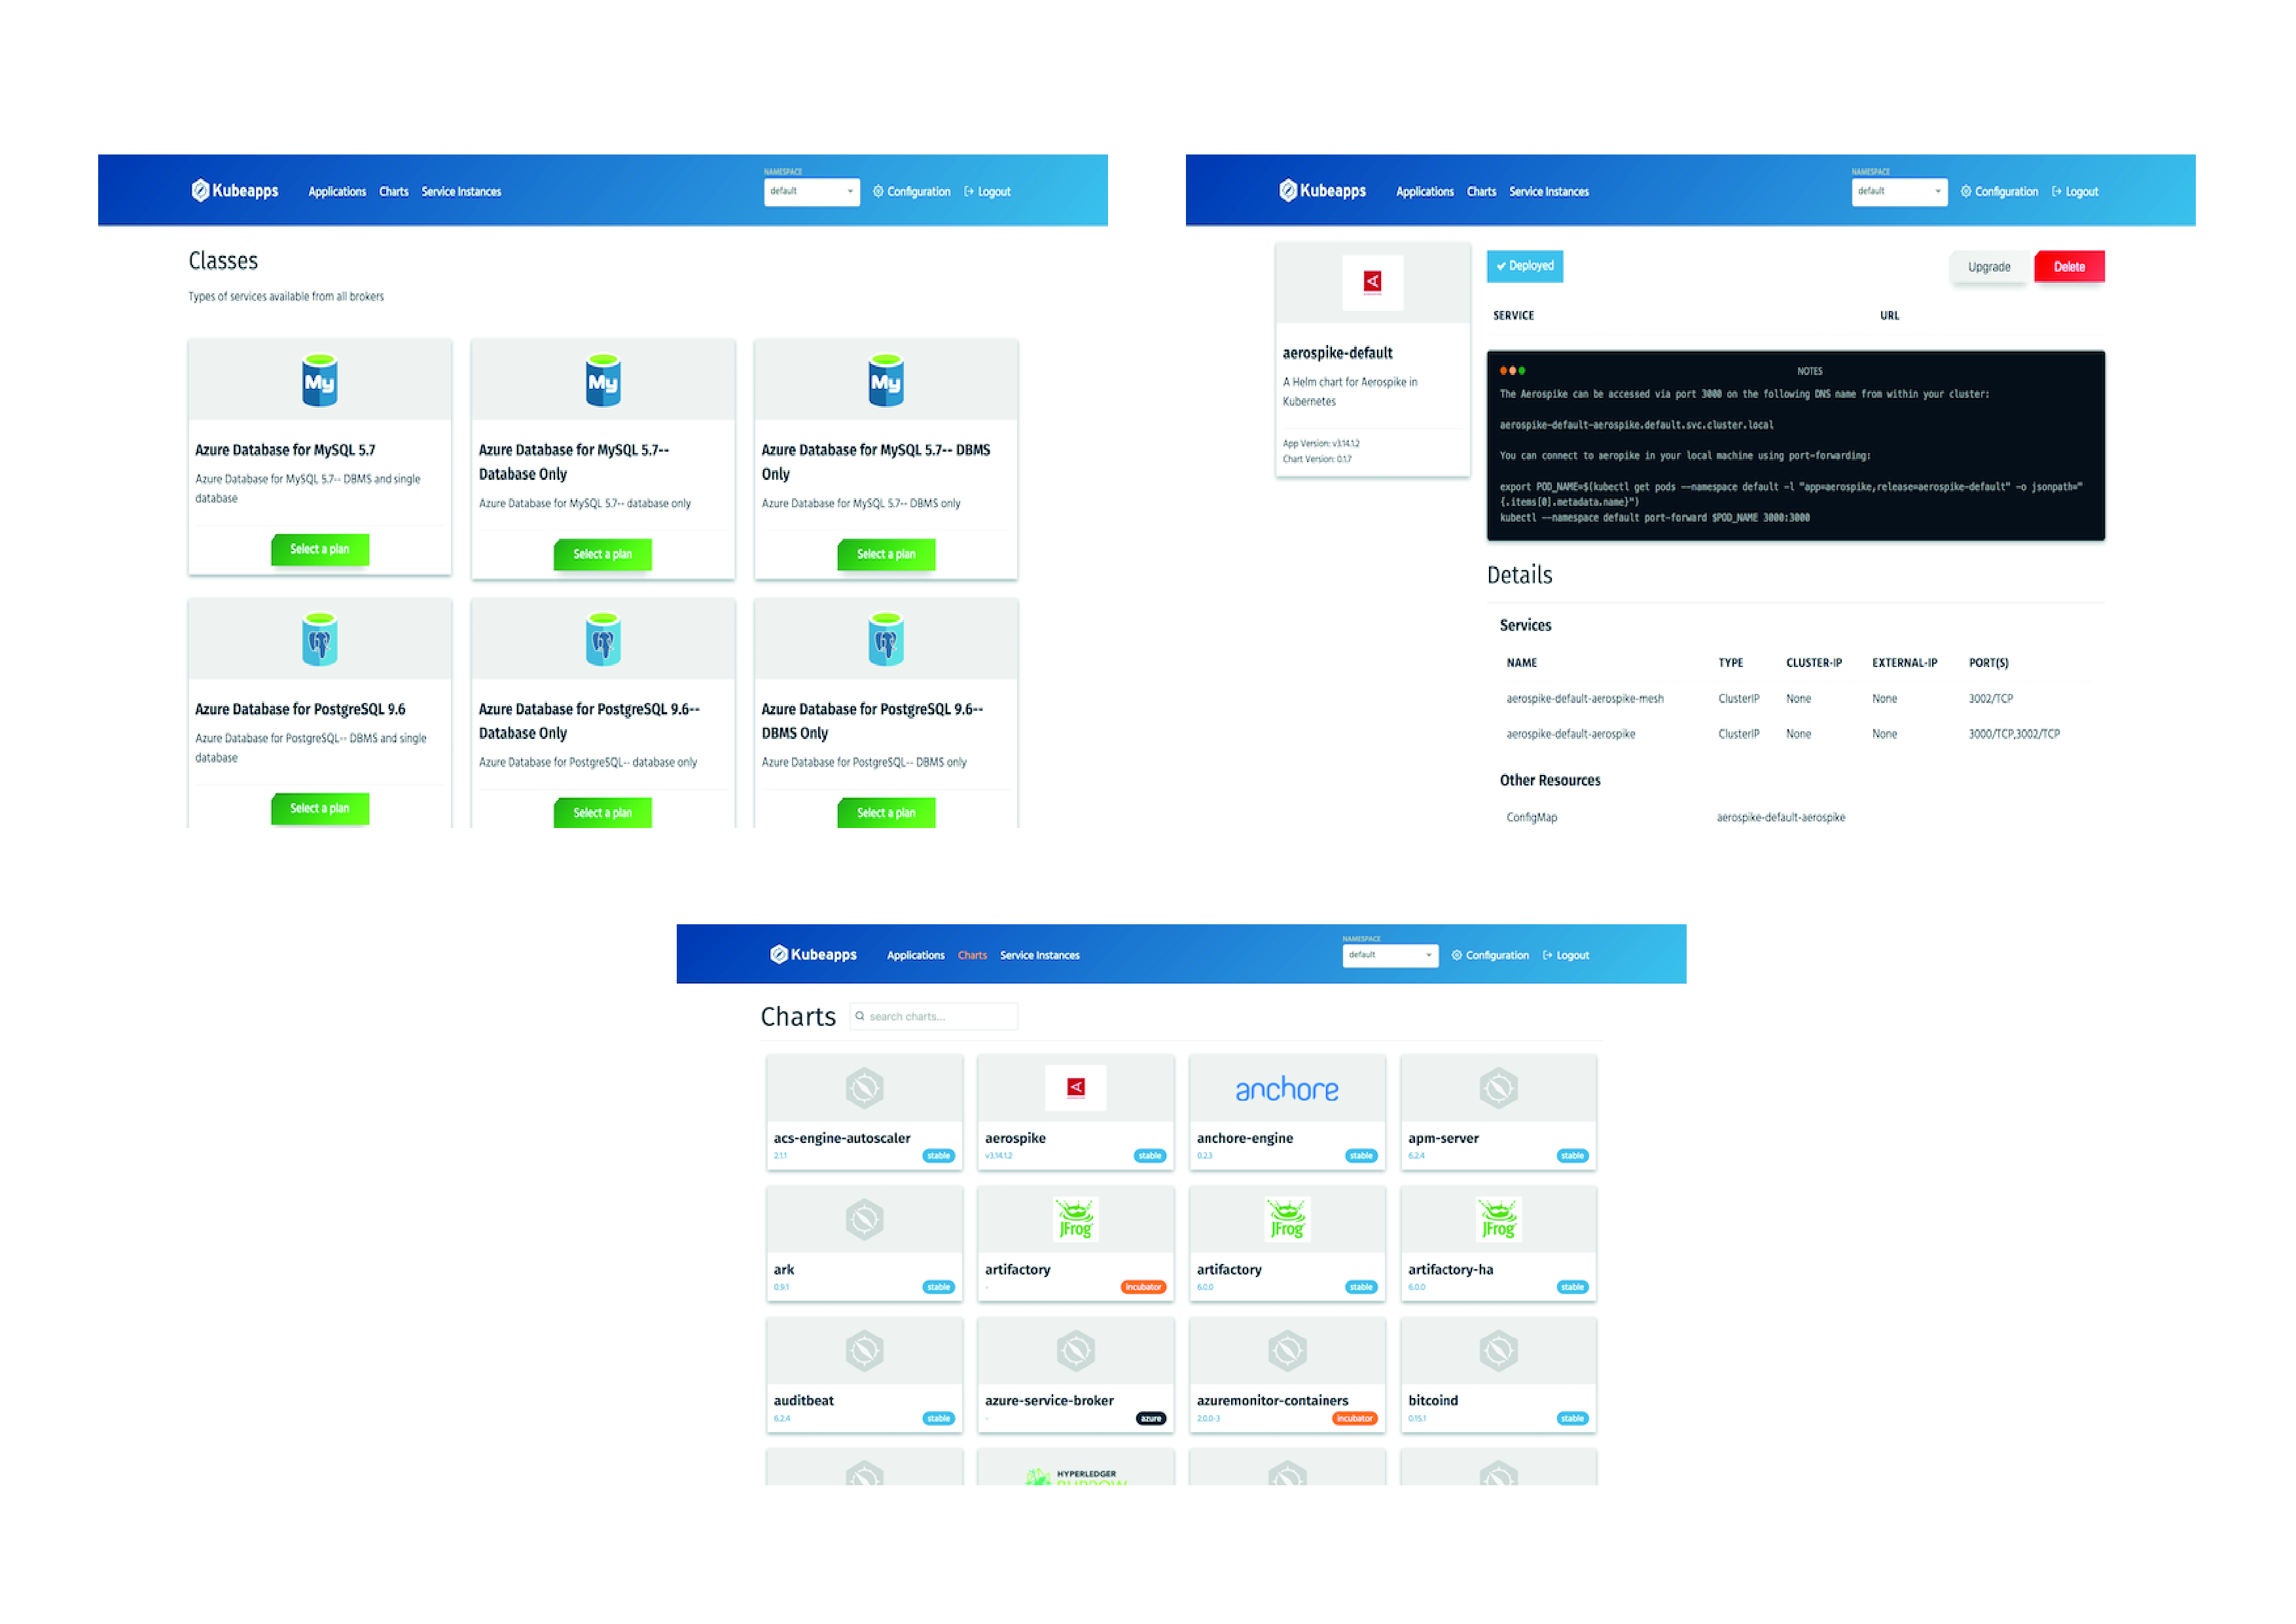
\includegraphics[scale=0.12]{Pictures/onyxia/kubeapps.jpg}
\captionsetup{margin=1.5cm,format=hang,justification=justified}
\caption[]{Aperçus de l'interface de kubeapps \newline}
\end{figure}

\paragraph{Architecture}
Kubeapps est une application respectant l'architecture microservice. Elle est composée d'une ihm écrite en react/javascript (Kubeapps dashboard). Mais également d'une api écrite en Go (Kubeops), elle est en charge de la communication avec l'API de helm 3 ou encore avec les différentes ressources kubernetes (comme les AppRepositories ou les secrets).\\

\paragraph{Verdict}
Kubeapps permet donc de faire une grosse partie de ce que onyxia fait : lister des services et les installer dans le cluster, consulter leur configuration et y accéder. Cependant ce dernier ne permet pas de forcer certaines valeurs à la place de l'utilisateur (par exemple l'url),  de plus kubeapps ne configure pas les services tout seul, c'est à l'utilisateur de saisir la configuration (pour un postgres il faudrait notamment que l'utilisateur choisissent son mdp, son url, la taille de la bdd associées etc...). Utiliser kubeapps comme une alternative à Onyxia n'est pas possible sans modifier son code source. Cela impliquerait de modifier le code de kubeops (l'api) écrit en go, mais le rapport coût d'entrée + développement est relativement élevé, et le go n'étant pas courant à l'Insee cela créerait une application difficilement maintenable.\\

Une deuxième solution a été de faire discuter onyxia directement avec l'API de kubeapps. En effet on pourrait déployer kubeapps dans le cluster faire dialoguer Onyxia avec Kubeapps. Cela permettrait au développeur de se connecter sur kubeapps à l'aide d'un token kubernetes et pouvoir configurer leur application tel qui le souhaite, et au statisticien d'utiliser onyxia pour déployer des services configuré rapidement. Onyxia devra donc être capable de forcer les values pour chaque déploiement. L'API de kubeapps nous servirait donc a installer le chart, à lister ceux déja déployer, et à les supprimer. 
\begin{figure}[H]
\renewcommand{\figurename}{Graphique}
\hspace{-3cm}
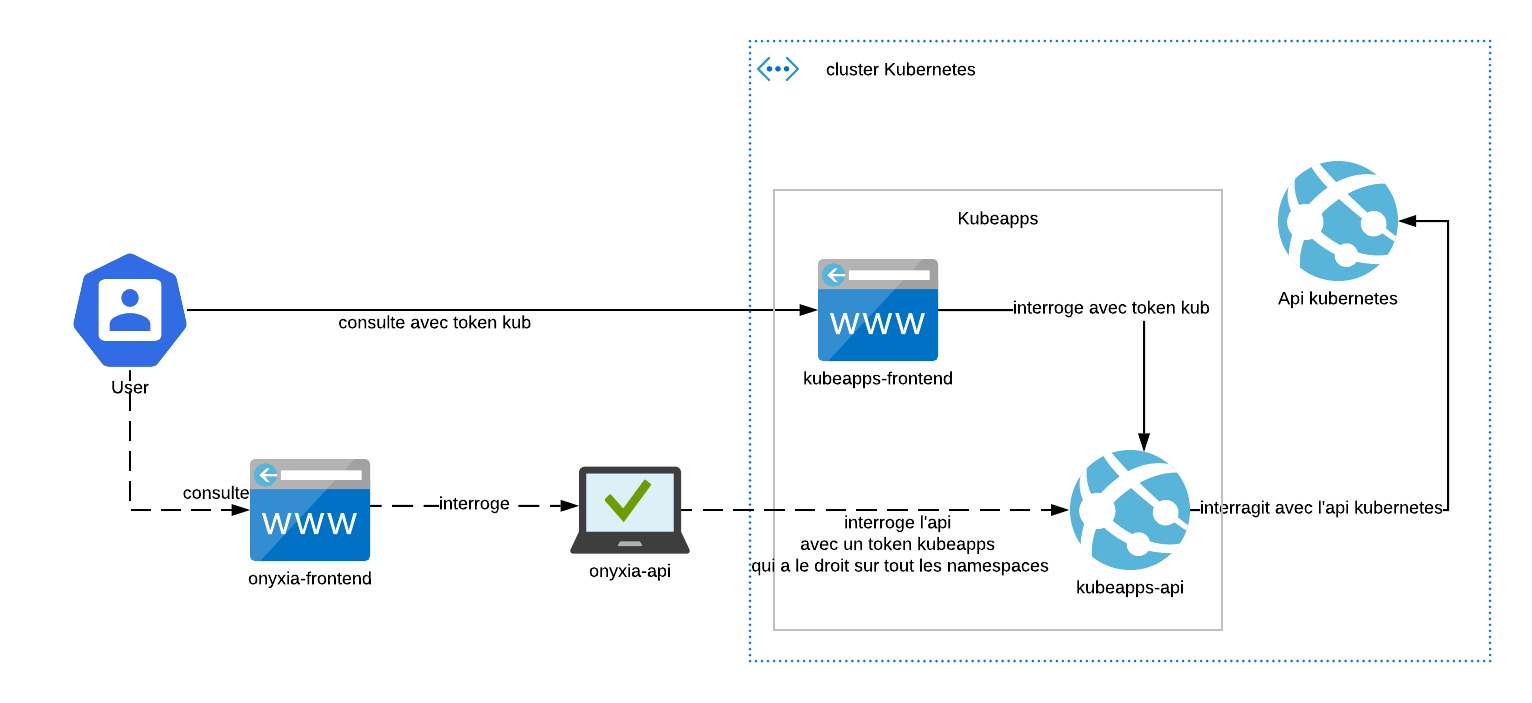
\includegraphics[scale=0.8]{Pictures/onyxia/kubeapps.png}
\captionsetup{margin=1.5cm,format=hang,justification=justified}
\caption[]{Architecture onyxia + kubeapps \newline}
\end{figure}

Cette solution n'a finalement pas été retenu, en effet faire reposer Onyxia sur kubeapps n'est pas forcement quelque chose de souhaitable puisque les différents endpoints de kubeapps peuvent être amenés à évoluer. De plus kubeapps devenait juste un intermédiaire entre helm et Onyxia, le cout pour qu'Onyxia  puisse dialoguer directement avec helm ne nous paraissant pas très important.



%----------------------------------------------------------------------------------------
%	BIBLIOGRAPHY
%----------------------------------------------------------------------------------------

\chapterimage{/chapter-image/bibliography.png}
\chapter*{Bibliographie}
\addcontentsline{toc}{chapter}{\textcolor{ocre}{Bibliographie}}
\nocite{*}
\vspace{-2cm}
\printbibliography[heading=bibempty]



%----------------------------------------------------------------------------------------
%	INDEX
%----------------------------------------------------------------------------------------

\cleardoublepage
\phantomsection
\setlength{\columnsep}{0.75cm}
\addcontentsline{toc}{chapter}{\textcolor{ocre}{Index}}
\printindex

%----------------------------------------------------------------------------------------

\end{document}
